\documentclass[magister]{dyplom} 

\usepackage[utf8]{inputenc}
\usepackage{hyperref}
\usepackage[toc]{appendix}
\usepackage{mathtools}
\usepackage{placeins}
\usepackage[nonumberlist,nopostdot]{glossaries}
\usepackage{listings}
\usepackage{amsmath}
\usepackage{xcolor}
\usepackage{pgf-umlsd}
\usepackage{subcaption}
\usepackage{tikz}
\usetikzlibrary{matrix,chains,positioning,decorations.pathreplacing,arrows}
\usepackage{minted}    
\usepackage{verbatim}

\numberwithin{listing}{section}

\titlen{Voice authentication library}
\author{Mariusz Pasek}
\promotor{dr Filip Zagórski}
\kierunek{Informatyka}
\specjalnosc{Computer Security}
\wydzial{Wydział Podstawowych Problemów Techniki}

\renewcommand{\figurename}{Fig.}

\makeindex
\makeglossaries
\newglossarystyle{mylong}{%
	\setglossarystyle{long}%
	\renewcommand{\glsgroupskip}{}
	\renewenvironment{theglossary}%
	{\begin{longtable}[l]{@{}p{\dimexpr 2cm-\tabcolsep}p{0.8\hsize}}}
		{\end{longtable}}%
	\renewcommand{\glsnamefont}[1]{\textbf{##1}}
}


\begin{document}
	\maketitle
	\tableofcontents
	\newglossaryentry{DSP}
	{
		name=DSP, 
		description={Digital Signal Processing}
	}
	\newglossaryentry{DFT}
	{
		name=DFT, 
		description={Discrete Fourier Transform}
	}
	\newglossaryentry{DTFT}
	{
		name=DTFT, 
		description={Discrete Time Fourier Transform}
	}
	\newglossaryentry{IDTFT}
	{
		name=IDTFT, 
		description={Inverse Discrete Time Fourier Transform}
	}
	\newglossaryentry{FFT}
	{
		name=FFT, 
		description={Fast Fourier Transform}
	}
	\newglossaryentry{T}
	{
		name=$T$, 
		description={Sampling period}
	}
	\newglossaryentry{base_freq}
	{
		name=$\omega_0$, 
		description={Base frequency}
	}
	\newglossaryentry{DAC}
	{
		name=DAC, 
		description={Digital to analog converter}
	}
	\newglossaryentry{FIR}
	{
		name=FIR, 
		description={Finished impulse response}
	}	
	\newglossaryentry{MFCC}
	{
		name=MFCC, 
		description={Mel frequency cepstral coefficient}
	}	
	\newglossaryentry{N_frame}
	{
		name=$N_{frame}$, 
		description={number of samples in processed frame}
	}
	\newglossaryentry{f_l}
	{
		name=$f_l$, 
		description={Lower bound of frequency used in mel filter bank generation in freq. domain}
	}	
	\newglossaryentry{f_h}
	{
		name=$f_h$, 
		description={Higher bound of frequency used in mel filter bank generation in freq. domain}
	}	
	\newglossaryentry{m_l}
	{
		name=$m_l$, 
		description={Lower bound of frequency used in mel filter bank generation in mel domain}
	}	
	\newglossaryentry{m_h}
	{
		name=$m_h$, 
		description={Higher bound of frequency used in mel filter bank generation in mel domain}
	}		
	\newglossaryentry{n_c}
	{
		name=$n_c$, 
		description={Number of \gls{MFCC} used}
	}			
	\newglossaryentry{epsilon}
	{
		name=$\varepsilon_f$, 
		description={Numerical epsilon for float numbers}
	}	
	\newglossaryentry{DCT}
	{
		name=DCT, 
		description={Discrete Cosine Transform}
	}
	\newglossaryentry{n_l}
	{
		name=$n_l$, 
		description={Number of liftered \gls{MFCC}}
	}	
	\newglossaryentry{V_n}
	{
		name=$V_n$, 
		description={Vector of extracted speaker features}
	}
	\newglossaryentry{CMS}
	{
		name=CMS, 
		description={Cepstral Mean Subtraction}
	}
	\newglossaryentry{N_frames}
	{
		name=$N_{frames}$, 
		description={Number of frames in processed sample}
	}
	\newglossaryentry{CDF}
	{
		name=CDF, 
		description={Cumulative Distribution Function}
	}
	\newglossaryentry{GMM}
	{
		name=GMM, 
		description={Gaussian Mixture Model}
	}
	\newglossaryentry{PCA}
	{
		name=PCA, 
		description={Principal Components Analysis}
	}
	\newglossaryentry{SVM}
	{
		name=SVM, 
		description={Suppor Vector Machine}
	}
	\newglossaryentry{WAV}
	{
		name=\texttt{WAV}, 
		description={Waveform File Format}
	}	
	\newglossaryentry{ASV}
	{
		name=\texttt{ASV}, 
		description={Automatic Speaker Verification}
	}	


	\glsaddall
	\printglossary[style=mylong,title=Acronyms and abbreviations]	
	
	\chapter{Introduction}
	
	The main goal of this thesis is to explain and implement techniques used during speaker verification process. The main applications of such algorithms are access control and transaction authentication \cite{OverviewOfSpeakerTechnology}. Moreover text independent speaker verification can be used to construct protocols that would contain also some sort of a challenge (like request to say specific combination of words) and therefore would not be vulnerable to simple replaying voice of the legitimate speaker. Automatic speaker verification does not require specialized hardware (as in the case of fingerprint verification), while preserving the advantages of biometric systems (like lack of password/PIN that could leak or be forgotten). \gls{ASV} is also often chosen as part of multilevel access control and it was deeply researched during last years \cite{SpeakerRecognition}.\\
	
	This thesis consists not only of theoretical background and explanation of the whole process, but also a source code of a library and simulation results that are proving effectiveness of presented methods. The library was written in \texttt{Python} and could be successfully used as a reference model during implementing such system in lower level languages.\\
	
	The part of the library that is responsible for classification of the speaker is also written in a flexible way that not only lets to include it in some other project, but also easily extend it by more specialized classification methods.
	
	\chapter{Digital Signal Processing}
	
	\section{General concept of DSP} \label{sec:general_concept_DSP}
	
	\gls{DSP} (Digital Signal Processing) deals of analyzing some streams of data. This data could be some physical measurements (like sound, electromagnetic wave readings, temperature, voltage, etc.), but it could be also incoming stream of encrypted or compressed data. In most of the cases, the data is coming from some kind of sensor (voltmeter, microphone). In such case it comes firstly in analog form and should be initially digitalized. Digitalization is a process that consists of two steps:
	
	\begin{itemize}
		\item Data should be sampled in time (time quantization),
		\item Values of each sample needs to be quantized as well (amplitude quantizetion).
	\end{itemize}
	
	\begin{figure}[!th]
		\centering
		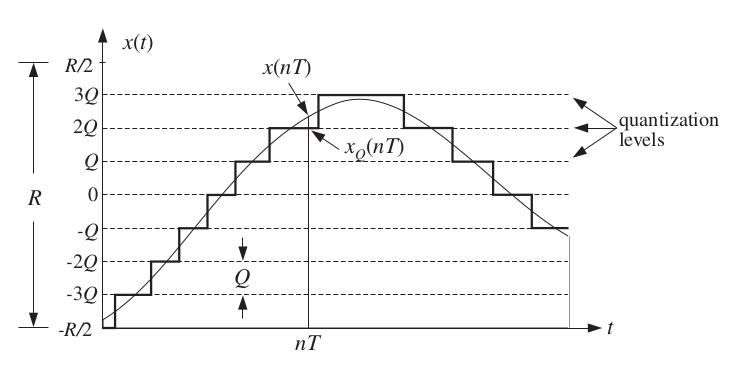
\includegraphics[width=0.7\linewidth]{images/quantization}
		\caption{Example quantization of analog signal \cite{IntroductionDSPBook}}
		\label{fig:quantization}
	\end{figure}

	
	Figure \ref{fig:quantization} shows some example process of quantizing analog signal. Quantization in time is about choosing some specific period (usually in \gls{DSP} denoted as \gls{T}) called sampling period. Each sample of incoming data is collected with this time interval. \\
	
	In order to store each sample in digital form it is also necessary to choose a specific range and number of bits that would define values of measured signal. This approach lets to store processed samples in electronic memory for later processing. It is of course clear that choosing specific minimal step between two samples implies necessity of rounding signal - i.e., loosing part of information. Another undesired phenomena is saturation. The signal is saturated, if its initial value exceeds defined range, i.e. cannot be expressed precisely in chosen notation.\\
	
	After the digitalized signal is processed it is also applied to many algorithms that are widely used during such processing (like filtering, windowing, convolving, etc.). Each of them has its own properties and some will be described later on in this chapter.\\
	
	The final stage of digital signal processing is giving an output of whole process. The output could be another stream of data (like decrypted data, decompressed image/audio stream) or single message (like identity of the speaker). All of these steps that are building \gls{DSP} chain are summarized in figure \ref{fig:typical_dsp_chain}.
	
	\begin{figure}[!th]
	\centering

	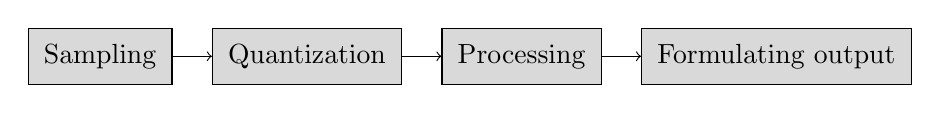
\begin{tikzpicture}[
		start chain,
		node distance=5mm, 
		every node/.style={draw,on chain,join,fill=gray!30,inner sep=2mm}, 
		every join/.style={->}
	]
		\node{Sampling};
		\node{Quantization};
		\node{Processing};
		\node{Formulating output};
	\end{tikzpicture}

	\caption{Typical DSP chain}
	\label{fig:typical_dsp_chain}
	\end{figure}
	
	\section{Fourier transform}
	
	\subsection{Theoretical background}
	
	Let us define harmonic (subcarrier) of the signal. Harmonic is some periodic function. If we defined the base frequency \gls{base_freq}, then we could say that frequency of any harmonic of order $k$ would be given by following equation:
	
	\begin{equation}	
		\omega_k = k \cdot \omega_0
	\end{equation}
	
	
	The subcarrier could be any periodical function, but the most widely used one is a sine wave \cite{IntroductionDSPBook}. Lets assume that we obtain following periodical signal:
	
	\begin{equation}
		\forall_t \  x(t) = x(t + T)
	\end{equation}
	
	
	Then we would like to express signal $x$ as a sum of its harmonics:
	
	\begin{equation} \label{eq:signal_synthezis}
		x(t) = \sum_{k = - \infty}^{\infty} c_k e^{jk\omega_0t} = \sum_{k = -\infty}^{\infty} c_k e^{jk2 \pi t / T}
	\end{equation}
	
	Where:
	
	\begin{itemize}
		\item $\omega_0 = \frac{2\pi}{T}$  -- base frequency,
		\item $c_k$ -- coefficients of harmonics,
		\item $T$ -- period of the signal.
	\end{itemize}
	
	With simple conversion of equation \ref{eq:signal_synthezis} we would obtain the following:
	
	\begin{align}
		\int_{T} x(t) e^{-jn\omega_0t} dt = \int_{T} \left( \sum_{k=-\infty}^{\infty} c_k e^{jk\omega_0t} \right) e^{-jn\omega_0t} dt = \nonumber \\		
		= \sum_{k=-\infty}^{\infty} c_k \left( \int_{T} e^{j(k-n)\omega_0t} dt \right)
	\end{align}
	
	It is worth to notice that:
	
	\begin{equation}
		\int_{T} e^{j(k-n)\omega_0t} dt = \begin{dcases}
										  T, \quad  k = n \\
										  0, \quad k \neq n
										  \end{dcases}
	\end{equation}
	
	This leads to conclusion:
	
	\begin{align}
		\int_{T} x(t) e^{-jk\omega_0t} dt = c_k T \\
		c_k = \frac{1}{T} \int_{T} x(t) e^{-jk\omega_0t} dt \label{eq:signal_analyzis}
	\end{align}
	
	Equation \ref{eq:signal_analyzis} shows how to calculate coefficients of harmonics of each order for a given periodical signal. It is easy to see that frequency of each subcarrier is given by equation $k \cdot \omega_0$. Thanks to trigonometrical expression of complex numbers:
	
	\begin{equation}
		e^{j\alpha} = cos(\alpha) + j sin(\alpha)
	\end{equation}
	
	it becomes clear that periodical signal $x$ is expressed by sum of sines and cosines (just as initially written in equation \ref{eq:signal_synthezis}). Fourier transform is linear operation that transforms periodical signal into its harmonic coefficients. Except for its continuous interpretation previously presented it has also its discrete form. It is called \gls{DFT} - Discrete Fourier Transform. It is given by following equations:
	
	\begin{equation} \label{eq:dft_synthezis}
		x_n = \sum_{k=0}^{N} c_k e^{jk\omega_0n}
	\end{equation}
	\begin{equation} \label{eq:dft_analyzis}
		c_k = \frac{1}{N} \sum_{k=0}^{N} x_n e^{-jk\omega_0n} 
	\end{equation}
	
	Where equation \ref{eq:dft_analyzis} describes analysis of given signal, while \ref{eq:dft_synthezis} describes synthesis. The most commonly used variation of this algorithm is \gls{FFT} (Fast Fourier Transform), which is an optimization of \gls{DFT}, but works basically the same \cite{IntroductionDSPBook}.
	
	\subsection{DFT basic properties}
	
	\subsubsection{DFT of simple functions}
	
	It can be easily noticed from figures \ref{fig:sine} - \ref{fig:rect_window} that signal in frequency domain is antisymmetric on the imaginary side and symmetric on the real side. This property is satisfied only for real signals. It basically means that if one is processing real signals (like sound) it is not necessary to store the whole output of \gls{DFT}. Instead of it one half could be skipped. This approach can let to optimize further computations and reduce memory consumption.\\
	
	Another relevant property is that odd functions in frequency domain have only imaginary component, while even functions have only real component. This is simple result of the fact that sine (imaginary part) is an odd function and cosine (real part) is even. 
	
	\begin{figure}[!th]
		\centering
		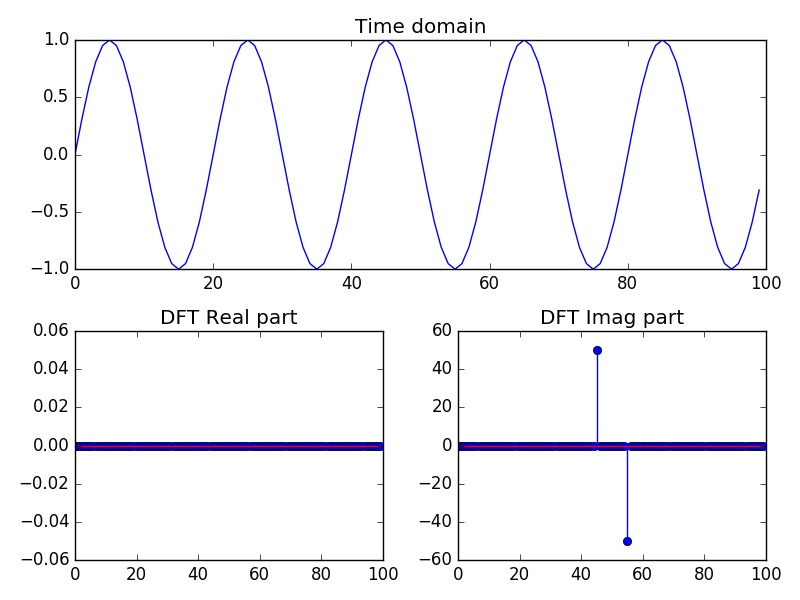
\includegraphics[width=0.7\linewidth]{images/sine}
		\caption{Sine function expressed in time and frequency domain}
		\label{fig:sine}
	\end{figure}

	\begin{figure}[!th]
		\centering
		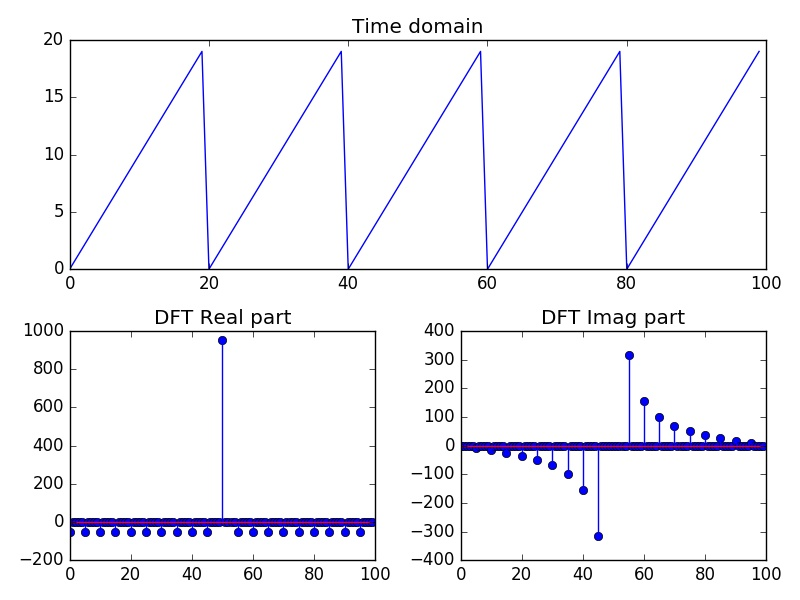
\includegraphics[width=0.7\linewidth]{images/saw}
		\caption{Sawtooth function expressed in time and frequency domain}
		\label{fig:saw}
	\end{figure}

	\begin{figure}[!th]
		\centering
		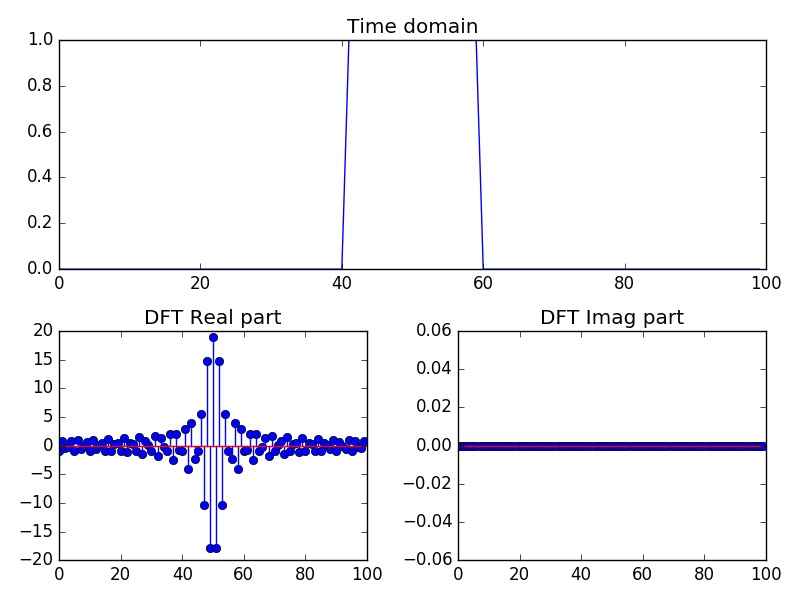
\includegraphics[width=0.7\linewidth]{images/rect_window}
		\caption{Rectangular window expressed in time and frequency domain}
		\label{fig:rect_window}
	\end{figure}

	
	\subsubsection{DFT of time shifted signal}
	
	Figure \ref{fig:sine_shifted} shows the result in frequency domain of shifting signal in time domain. The shifted sine function is not fully imaginary anymore. Instead of it part of its imaginary part has moved into the real part (absolute value has left the same). This is the result of rotation of samples of \gls{DFT}. This is very important property in \gls{DSP}. It sounds as follows: every cyclic shift in time domain results with rotation in frequency domain and vice versa.
	
	\begin{figure} [!th]
		\centering
		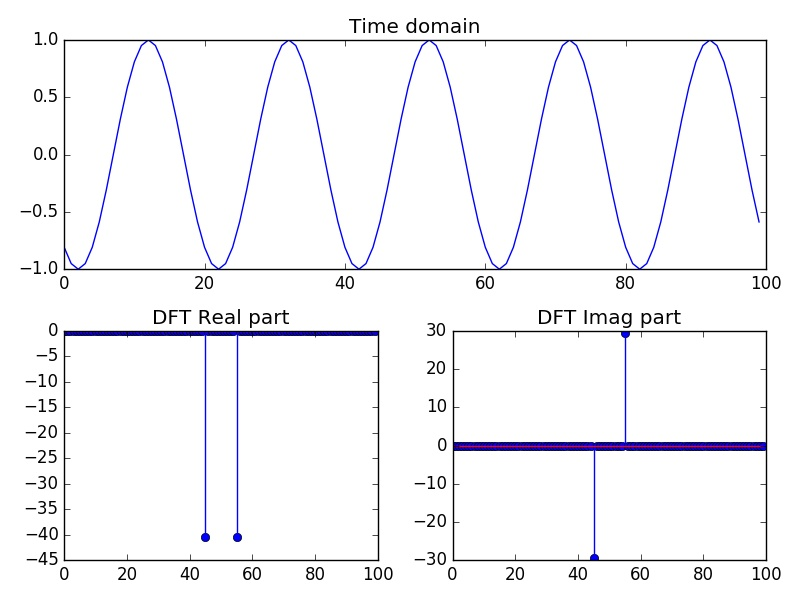
\includegraphics[width=0.7\linewidth]{images/sine_shifted}
		\caption{Shifted sine function expressed in time and frequency domain}
		\label{fig:sine_shifted}
	\end{figure}

	
	\subsubsection{DFT of two multiplied signals}

	Figure \ref{fig:m_sine_rect} shows the result of simple multiplication of sine wave and rectangular window. The frequency domain seems to be very distorted and hard to recognize as spectrum of sine function. This is the effect of another important \gls{DFT} property. Multiplication of signals in one domain results in convolution in another. Convolution of discrete, finite signals is given by equation:
	
	\begin{equation}
		(f * g)[n] = \sum_{m=0}^{N-1} f[m] g[n-m]
	\end{equation}

	Knowing this property lets to easily explain the output of \gls{DFT} of multiplying sine wave with rectangular window. This distortion can lead to serious mistakes during later processing of the signal and that is the reasoning for using different windows than rectangular.

	\begin{figure} [!th]
		\centering
		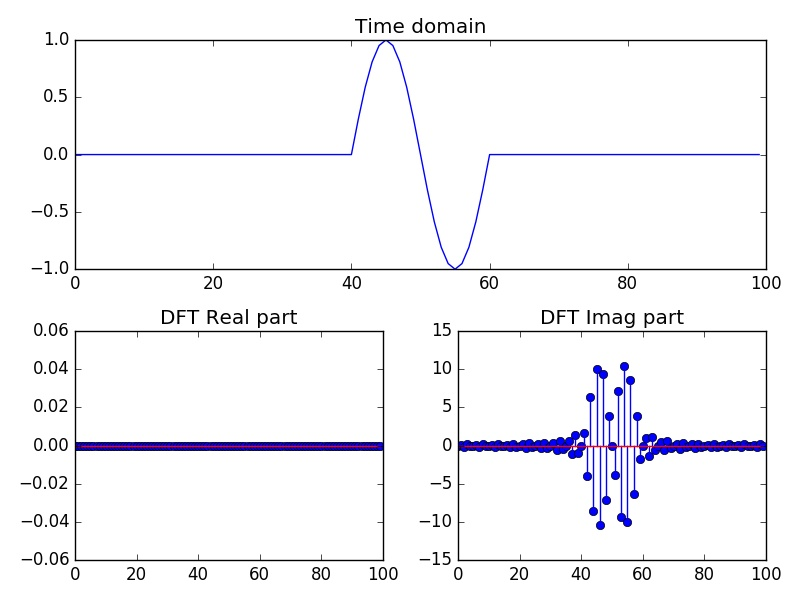
\includegraphics[width=0.7\linewidth]{images/m_sine_rect}
		\caption{Sine function multiplied by rectangular window expressed in time and frequency domain}
		\label{fig:m_sine_rect}
	\end{figure}

\FloatBarrier
	
	\section{Sampling theorem}	

	As mentioned in section \ref{sec:general_concept_DSP}, the first step of digital signal processing is sampling it. In order to sample analog signal it is necessary to choose sampling period. It is a trade-off between resources consumption and precision. Too short sampling period could lead to unnecessary increase of memory consumption and could even make impossible achieving assumed performance (like real time processing). On the other choice of too long sampling period could lead to loss of relevant information.\\
	
	One of the assumptions about signals in \gls{DSP} is that their spectrum remains constant in some short period (like single radio symbol during wireless transmissions or single tone during speech processing). This means that collected samples are sorted in groups of the same size (lets define them as frames). In order to choose \gls{T} properly one should pick it in such a way that it would be possible to calculate the amplitude of the subcarrier of the highest possible frequency. The equation that defines minimal frequency of sampling - $f_s$ that lets to calculate amplitude of some maximal harmonic (of frequency $\omega_m$) is called Nyquist criterion. It is presented in the equation \ref{eq:nyq_criterion}:
	
	\begin{equation} \label{eq:nyq_criterion}
		f_s = 2 \cdot \omega_m
	\end{equation}
	
	If one would try to calculate \gls{DFT} of the signal without following Nyquist criterion it would be impossible to distinguish signals of some frequencies just as presented in figure \ref{fig:aliasing}. \\
	
	\begin{figure} [!th]
		\centering
		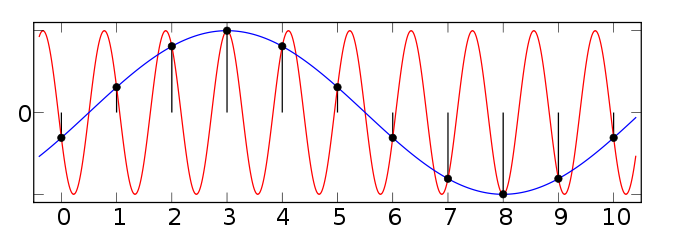
\includegraphics[width=0.7\linewidth]{images/aliasing}
		\caption{Phenomena of aliasing \cite{aliasing_wikipedia}}
		\label{fig:aliasing}
	\end{figure}
	
	Phenomena of aliasing causes the sensor with insufficient sampling frequency to register signals of lower frequencies that were never actually received. Instead these are just decimated signals of higher frequencies that were impossible to be registered because of not following Nyquist criterion.\\
	
	In order to prevent this phenomena to happen it is necessary to apply low pass analog filters that can exclude signals of high frequencies before sampling. Therefore any \gls{DAC} (digital to analog converter) uses such filter as a first step of conversion. Since the subject of this thesis is just to process digital signals and whole conversion is provided by microphone and computer sound card it is not necessary to prevent aliasing occurrence.

	\section{Windowing}
	
	Since during \gls{DSP} we are processing just somehow preprepared frames, we need to handle some kind of windowing. It basically means that one should try to minimize spectrum distortion caused by dealing with only some part of the signal instead of its full period. Such situation causes phenomena called "spectrum leakage". It occurs if length of processed signal is not an integer multiplication of its period and leads to significant distortion of the original signal. The phenomena of spectrum leakage is presented in figure \ref{fig:sub_sine}.
	
	\begin{figure} [!th]
		\centering
		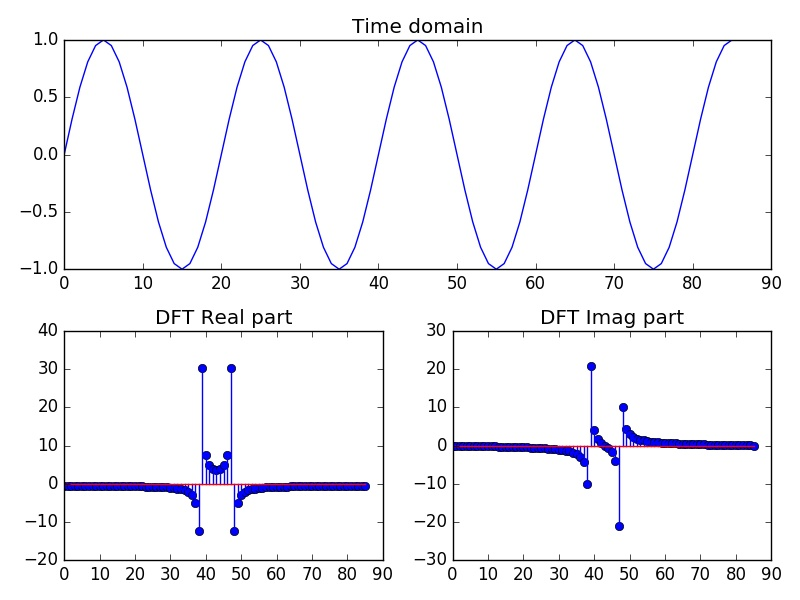
\includegraphics[width=0.7\linewidth]{images/sub_sine}
		\caption{Result of calculating dft of not integer number of periods -- spectrum leakage}
		\label{fig:sub_sine}
	\end{figure}

	
	 This is more or less the result of rectangular windowing. The way of minimizing this phenomena is to apply windows with more smooth edges. There are several windows widely used in \gls{DSP} and one of the most popular is Hamming window. It is given by the equation:
	
	\begin{equation}
		w(n) = \alpha - \beta \ cos \left( \frac{2\pi n}{N - 1} \right)
	\end{equation}
	
	where:
	
	\begin{itemize}
		\item $\alpha = 0.54$
		\item $\beta = 1 - \alpha = 0.46$
		\item $N$ is a number of samples in frame
	\end{itemize}
	
	The plot presenting Hamming window generated by given equation can be seen in figure \ref{fig:hamming}. And the result of multiplying signal from figure \ref{fig:sub_sine} by presented Hamming window is shown in figure \ref{fig:h_sub_sine}. \\
	
	\begin{figure} [!th]
		\centering
		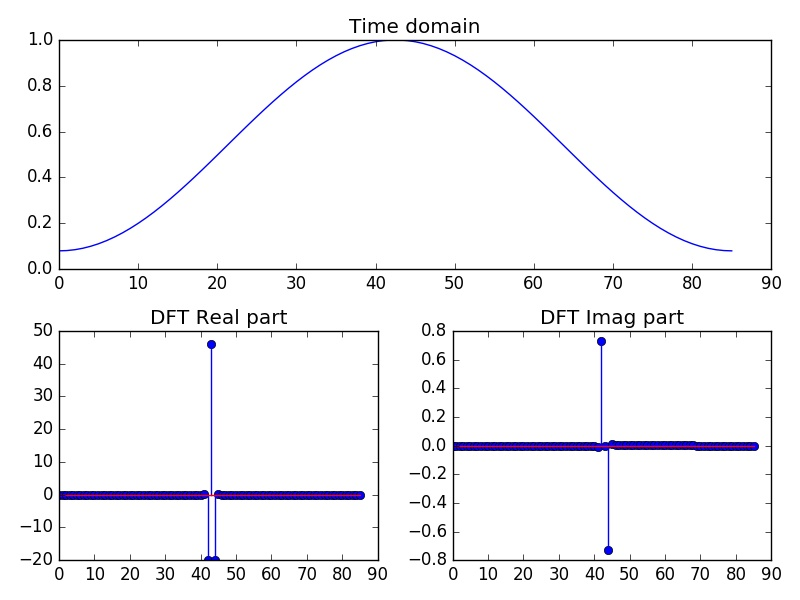
\includegraphics[width=0.7\linewidth]{images/hamming}
		\caption{Hamming window}
		\label{fig:hamming}
	\end{figure}
	
	\begin{figure} [!th]
		\centering
		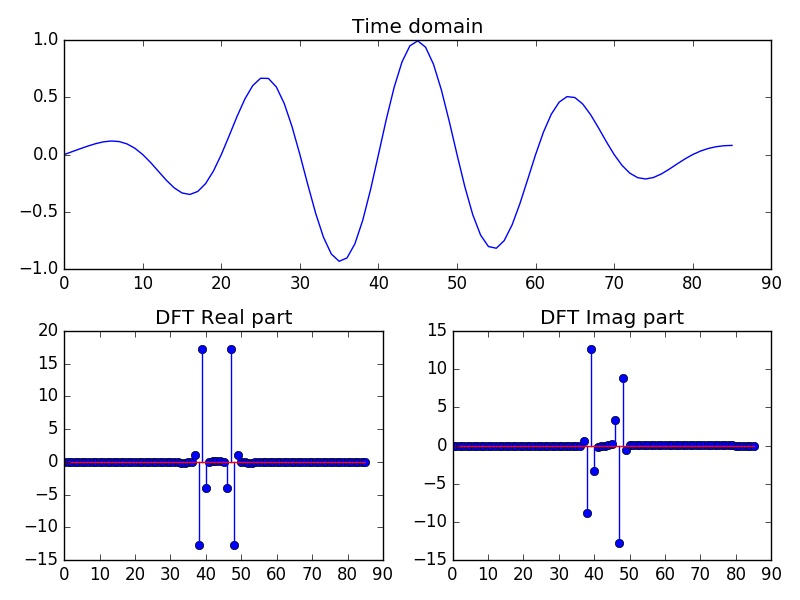
\includegraphics[width=0.7\linewidth]{images/h_sub_sine}
		\caption{Not integer number of sine periods multiplied by hamming window}
		\label{fig:h_sub_sine}
	\end{figure}

	It can be noticed that side peaks where not eliminated completely, but thanks to this solution it was possible to minimize effect of spectrum leakage. This phenomena was a motivation of using Hamming window as the first step of signal processing in cepstral analysis described in chapter \ref{sec:feature_extraction}.
	
	\FloatBarrier
	
	\section{Digital filters}
	
	Filtering is one of the most commonly used functionality provided by \gls{DSP}. The basic task of filter is to shape the spectrum of processed signal in a desired way by multiplying its by filter's spectrum. There are several basic types of filters:
	
	\begin{itemize}
		\item lowpass filter,
		\item highpass filter,
		\item bandpass filter,
		\item bandstop filter.
	\end{itemize}
	
	\begin{figure}
		\centering
		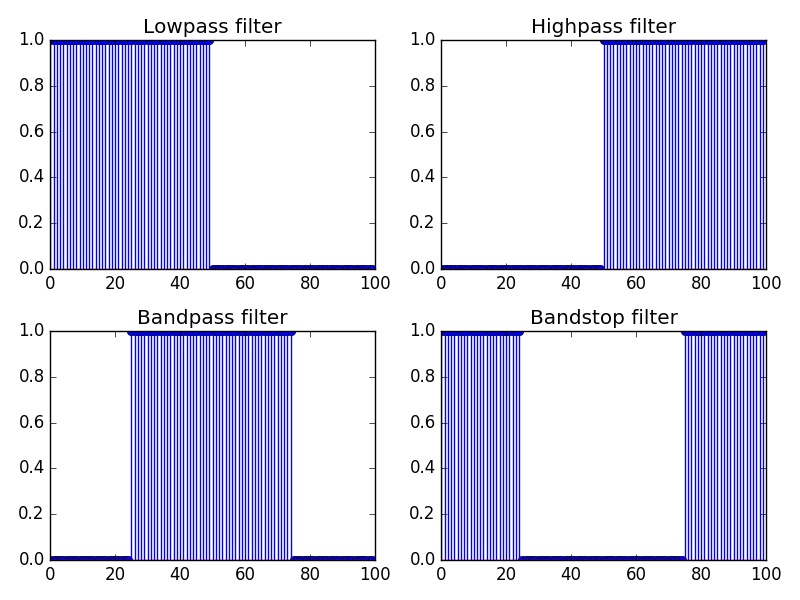
\includegraphics[width=0.7\linewidth]{images/filters_spectrum}
		\caption{Spectral presentation of basic filter types}
		\label{fig:filters_spectrum}
	\end{figure}
	
	The spectral presentation of these filters is shown in figure \ref{fig:filters_spectrum}. It can be easily seen that changes in these filters are rectangular -- are perfectly sharp. In real case scenarios it is not possible, to obtain such efficiency of filters in feasible computation time. That is why these filters are considered to be ideal, and commonly used filters are approximations of these. Since samples are firstly usually processed in time domain it would be convenient to map desired filter into some array of coefficients that would correspond to its spectral form. These coefficients must be convolved with incoming samples (because of basic \gls{DFT} properties). One can write down following equation:
	
	\begin{equation}
		y(n) = \sum_{i=0}^{M-1} x(n-i) \cdot c(i)		
	\end{equation}
	
	Where:
	
	\begin{itemize}
		\item $c$ -- filter coefficients,
		\item $M$ -- order of the filter.
	\end{itemize}
	
	It is not the only possible form of filtering, but one of most widely used. Order of the filter defines complexity of filtering and number of samples that need to be stored. Filters of this kind are called \gls{FIR} (finished impulse response) filters. This name is corresponding to very important property of such filter. The length of output on any input signal is never longer than $M$ samples. It is worth to notice that if one would put Dirac's delta as an $x(n)$ signal, the output would be $c(n)$. It is very important property that lets to check coefficients of some unknown \gls{FIR} filter. It is not the only kind of filter used in \gls{DSP}, but only such is used in this thesis.
	
	\subsubsection{Ideal filter impulse response}
	
	As it was mentioned previously, the generally used filters are just approximation of ideal ones. It is necessary then to find the coefficients of ideal filter. One could start with lowpass filter. Its ideal frequency response $H(\omega)$ is bounded to its impulse response $h(k)$ by \gls{DTFT} and \gls{IDTFT} relationships \footnote{It may seem confusing that the \gls{DTFT} relation is used in this consideration, but it is necessary. \gls{DFT} assumes that signal is sampled and quantized, while \gls{DTFT} assumes only sampling, and allows the signal change continuously and it results with spectrum being continuous function, i.e. such case is more general. Derivation of \gls{DTFT} equations was not covered in this thesis, but is analogous to \gls{DFT}.}:
	
	\begin{equation}
		H(\omega) = \sum_{n = -\infty}^{\infty} h(n) e^{-j\omega n}		
	\end{equation}
	\begin{equation}
		h(n) = \frac{1}{2 \pi} \int_{-\pi}^{\pi} H(\omega) e^{j\omega n} d \omega
	\end{equation}
	
	Since time coefficients of filters are considered to be real numbers, their spectral forms shown in figure \ref{fig:filters_spectrum} can be treated as symmetrical over vertical axis. Therefore one could define $H(\omega)$ of the lowpass filter in the following way:
	
	\begin{equation}
		H(\omega) = \begin{dcases}
						1, -\omega_c \leq \omega \leq \omega_c \\
						0, (-\pi \leq \omega < -\omega_c) \  \vee \ (\omega_c < \omega \leq \pi)
					\end{dcases}
	\end{equation}
	
	It lets to calculate impulse response of ideal lowpass filter:
	
	\begin{align} \label{eq:lowpass_impulse_response}
		h(n) = \frac{1}{2\pi} \int_{-\pi}^{\pi} H(\omega) e^{j \omega n} d \omega =  \frac{1}{2\pi} \int_{-\omega_c}^{\omega_c} 1 \cdot e^{j \omega n} d \omega = \nonumber \\ = \left[ \frac{e^{j\omega n}}{2\pi j n} \right]^{\omega_c}_{-\omega_c} = \frac{e^{j\omega_c n} - e^{-j\omega_c n}}{2\pi j n} = \nonumber \\ = \frac{cos(\omega_c n) + j sin(\omega_c n) - (cos(\omega_c n) - j sin(\omega_c n))}{2\pi j n} = \nonumber \\ = \frac{sin(\omega_c n)}{\pi n}
	\end{align}
	
	As it was shown in equation \ref{eq:lowpass_impulse_response}, the impulse response of lowpass filter ($h_{lowpass}(n, \omega_c)$) is given by sinc function (presented in figure \ref{fig:sinc}). Having impulse response of single lets to obtain impulse responses for other ideal filters. Having in mind that Dirac's delta spectral form is a sequence of ones lets to write the following equations \cite{IntroductionDSPArticle}:
	
	\begin{itemize}
		\item $h_{highpass}(n, \omega_c) = \delta(n) - h_{lowpass}(n, \omega_c)$
		\item $h_{bandpass}(n, \omega_a, \omega_b) = h_{lowpass}(n, \omega_b) - h_{lowpass}(n, \omega_a)$
		\item $h_{bandstop}(n, \omega_a, \omega_b) = \delta(n) - h_{bandpass}(n, \omega_a, \omega_b)$
	\end{itemize}
	
	\begin{figure}
		\centering
		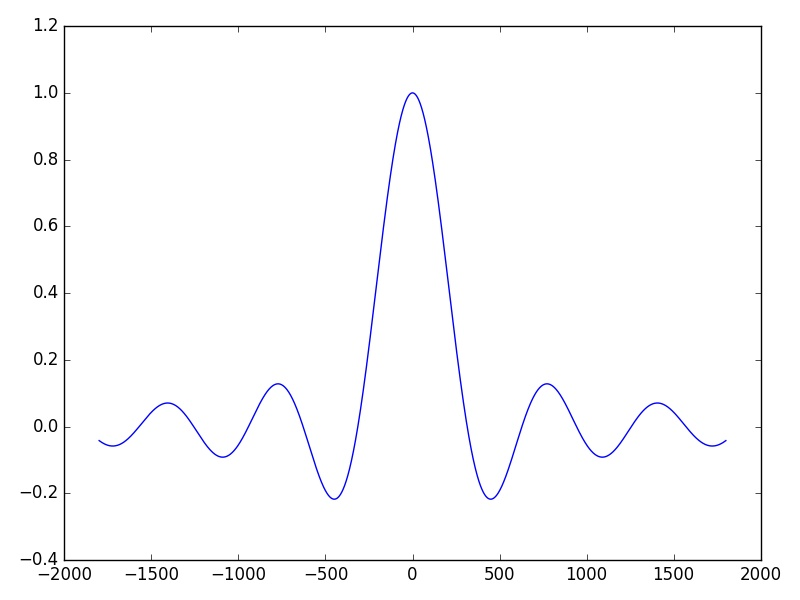
\includegraphics[width=0.7\linewidth]{images/sinc}
		\caption{Sinc function}
		\label{fig:sinc}
	\end{figure}
	
	\subsubsection{Designing FIR filters}
	
	Until now domain of $n$ was all integer numbers. In order to obtain feasible FIR filter one has to limit its order to some specific $M$. There are many approaches to do so. One of the most basic is rectangular window. This method composes of two steps. Truncating symmetrically impulse response and shifting it to only positive part. Truncating is necessary to reduce the order of the filter and shifting must be done for all real time applications, because it is impossible to get the value of future samples. \\
	
	Rectangular window is not only one used for designing FIR filters. Hamming and Kaiser windows are used as well and each of them have unique impact on behavior of signal processing, but all of these are using the same theoretical basis already described in this chapter.
	
	\chapter{Speaker recognition and voice authorization} \label{ch:speaker_recognition}
	
	\section{General approach of speaker recognition and voice authorization}
	
	Speaker recognition process is generally divided into three steps:
	
	\paragraph{Feature extraction} -- it is necessary in order to extract only relevant data from incoming signal that are characterizing particular speaker (or some specific sound generated by him -- like single vowel). In order to do so, one must divide stream of input into some smaller groups (frames). Every single frame should be considered as a single sound -- vowel in this case. It basically means that the output of feature extraction should be some coefficients that would characterize this frame.
	
	\paragraph{Classification} -- after extracting feature from the frame one should classify it, in order to determine if it is recognized as some known vowel of previously defined speaker. This is the second step of speaker recognition and it is somewhat independent on the first.
	
	\paragraph{Decision} -- having each frame classified lets to summarize collected information and finally decide, if stream of data was generated by known speaker or not. Decision block could also use some previous knowledge like information, about this, what the speaker actually said.

	\begin{figure}[!th]
		\centering
		
		\tikzstyle{block} = [draw, fill=gray!3, rectangle, minimum height=3em, minimum width=6em]
		\tikzstyle{sum} = [draw, fill=gray!3, circle, node distance=1cm]
		\tikzstyle{input} = [coordinate]
		\tikzstyle{output} = [coordinate]
		\tikzstyle{pinstyle} = [pin edge={to-,thin,black}]
		
		\begin{tikzpicture}[auto, node distance=2cm]
		\node [block, fill=gray!30] (paralleliser) {Stream to frames};
		\node [block, fill=gray!30, right of=paralleliser, node distance=4cm] (extractor1) {Extractor 1};		
		\node [block, fill=gray!30, right of=extractor1, node distance=3.5cm] (classifier1) {Classifier 1};
		\node [block, fill=gray!30, right of=classifier1, node distance=4cm] (decider) {Decision block};
		
		\node [block, fill=gray!30, below of=extractor1] (extractor2)   {Extractor 2};
		\node [block, fill=gray!30, below of=classifier1] (classifier2) {Classifier 2};

		\node [block, fill=gray!30, below of=extractor2, node distance=2.5cm] (extractorN)   {Extractor n};
		\node [block, fill=gray!30, below of=classifier2, node distance=2.5cm] (classifierN) {Classifier n};		
				
		\draw [->] (paralleliser) -- node[name=u] {} (extractor1);
		\draw [->] (extractor1) -- (classifier1);
		\draw [->] (classifier1) -- node [name=y] {}(decider);

		\draw [->] (u) |- (extractor2);
		\draw [->] (u) |- (extractorN);
		
		\draw [->] (extractor2) |- (classifier2);
		\draw [->] (extractorN) |- (classifierN);		

		\draw [-] (y) |- (classifier2);		
		\draw [-] (y) |- (classifierN);		
		
		\draw[dotted] (extractor2) -- (extractorN);
		\draw[dotted] (classifier2) -- (classifierN);		

		\end{tikzpicture}
		
		\caption{Speaker recognition algorithm}
		\label{fig:speaker_recognition_algorithm}
	\end{figure}
	
	\subsection{Voice authorization}
	
	Voice authorization algorithm could be used as part of an authorization tool, but it is not enough. In real case scenario one should protect from replay attacks. It would be very easy to record voice of a person and then play it again, to use it as authorization sequence. That is why real voice authorization mechanism should compose of following procedures:
	
	\begin{itemize}
		\item challenge -- verifier (Victor) queries prover (Peggie) with some sequence (some sentence for instance),
		\item response -- prover Peggie replies with its answer,
		\item verification -- finally Victor verifies an answer with two algorithms:
		\begin{itemize}
			\item Speaker recognition -- Victor checks, if given sentence was told by predefined person. It uses algorithm steps previously described in this chapter,
			\item Speech recognition -- Victor checks, if Peggie has told exactly, what was demanded in challenge. It is not the subject of this thesis, but there are many available ready solutions for this functionality (like one provided by \texttt{Google}).
		\end{itemize}		
	\end{itemize}	
	
	\begin{figure}[!th]
		\centering	
		\begin{sequencediagram}
			\newthread[white]{c}{Victor}
			\newinst[4]{s}{Peggy}
			
			\mess{c}{Challenge}{s}
			\mess{s}{Spoken sequence}{c}
			\mess{c}{Decision}{s}
			
		\end{sequencediagram}	
		\caption{Voice authorization message sequence}
		\label{fig:voice_authorization}
	\end{figure}
	
	\section{Feature extraction} \label{sec:feature_extraction}	
	
	As previously described, the first step of speaker recognition is extraction of speaker features from incoming signal. There are many approaches of this action, but one that became the most popular (as well in speech and speaker recognition systems) is \gls{MFCC} extraction. It bases on similar way of processing that human ear does and it is calculated in following steps:
	
	\begin{enumerate}
		\item pre-emphasis,
		\item decimation,
		\item frame division and operations computed per frame:
		\begin{enumerate}
			\item zero padding,
			\item applying \gls{FFT},
			\item conversion into mel scale,
			\item applying \gls{DCT},
			\item liftering,
			\item vector enhancements,		
		\end{enumerate}		
		\item appending deltas,
		\item cepstral mean subtraction,
		\item feature warping
	\end{enumerate}
	
	\subsection{Pre-emphasis}
	
	It has been researched that speaker features are being kept by higher frequencies of incoming signal. Therefore if one does not want to focus on information that was actually said by the speaker, but wants to focus only on his identity, it is necessary, to process the signal with highpass filter. The coefficients of applied filter are as following:
	
	\begin{itemize}
		\item $c_0 = 1$
		\item $c_1 = -0.97$
	\end{itemize}
	
	These values of pre-emphasis filter are usually used in publications treating about speaker recognition \cite{SpeakerIdentificationPresentation}. An example of pre-emphasis is shown in figure \ref{fig:MFCC_preemphase}. An initial signal is composed of low frequency sine wave and high frequency random noise. Filtering is canceling sine element of signal leaving only random noise.
	
	\begin{figure}[!th]
		\centering
		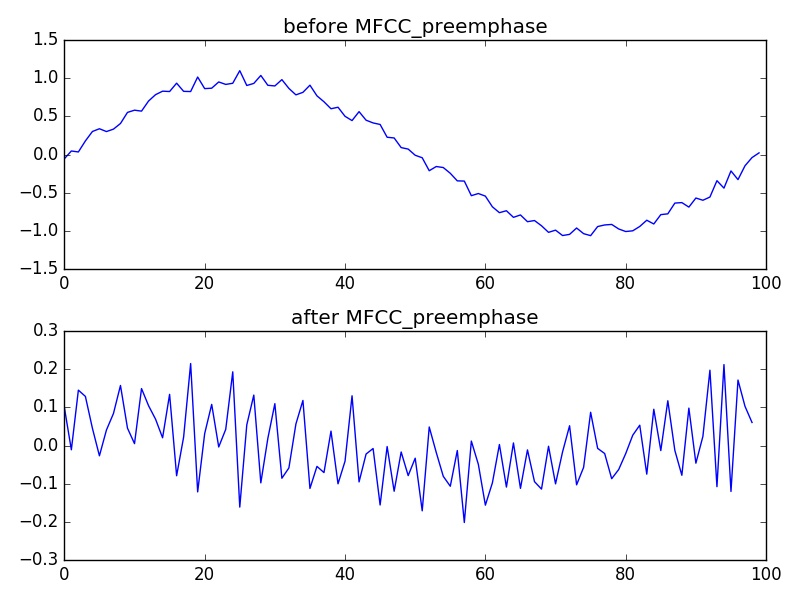
\includegraphics[width=0.7\linewidth]{images/MFCC_preemphase}
		\caption{Example of pre-emphasis high band filter application}
		\label{fig:MFCC_preemphase}
	\end{figure}

	
	\subsection{Decimation}
	
	It is not a required step, but it can be essential, if it is necessary to process signals sampled with various frequencies and for optimization purposes. Decimation is an algorithm that skips desired part of samples and therefore it reduces the frequency of sampling the signal. It lets to reduce number of processed samples (with simultaneous reduction of accuracy) and can let to normalize frequency of sampling of all incoming signals (regardless of the quality of them in the first place).
	
	\subsection{Frame division}

	As it was previously presented in figure \ref{fig:speaker_recognition_algorithm}, an incoming signal must be divided into single frames. The only thing that needs consideration during framing division are two parameters: frame length and frame step.
	
	\paragraph{Frame length} -- the length of the frame must be optimized in such a way that it would be highly probable to correspond, to the length of processed vowels (or at least part of them). It should never be to long, because in such case an algorithm would process data containing two vowels simultaneously. In speaker recognition algorithms this parameter was empirically determined as 25 ms. 
	
	\paragraph{Frame step} -- it is probable that single vowel would not exactly fit into one frame even if its length would be exactly the same, because it can be shifted. That is why it is also necessary to define frame step separately in order to increase probability of positive detection. It is also trade-off between accuracy of computation and optimization of an algorithm. The value of frame step in publications dealing with speaker recognition problem is 10 ms \cite{MFCC_description}. 
	
	\subsection{Zero padding}
	
	Since \gls{FFT} is optimization of \gls{DFT} algorithm that works most efficiently if applied on signals of length of power of 2, it can be necessary to extend the length of frames in such a way that their length would satisfy this condition. It is done by simple zero padding that is a neutral operation for \gls{DFT} algorithm.
	
	\subsection{Applying Fast Fourier Transform}	
	
	As mentioned previously, digital signal processing is much more comfortable in frequency domain. Therefore each zero padded frame must be transformed with \gls{FFT}.
	
	\subsection{Conversion into mel scale}
	
	Mel filtering is the essential part of \gls{MFCC} extraction. The general purpose of this step is to reduce amount of information held by samples. Depending on sampling frequency and decimation factor the frame can be of length 256, 512, 1024, etc. samples. Mel filtering lets to reduce these significant numbers into less than 30. \\
	
	It was discovered that human ear is distinguishing frequencies in logarithmic manner. Mel scale is a representation of the signal that is converting any signal into the same coefficients that are calculated by human ear. This conversion consists of following parameters:
	
	\begin{itemize}
		\item frequency range (\gls{f_l}, \gls{f_h})-- this is the range of frequency that is considered to contain all features of the speaker. It is usually defined as (15 Hz, 4 kHz),
		\item number of coefficients (\gls{n_c})-- this is a number into which length of each frame will be reduced. Value 26 is often picked for this parameter.
	\end{itemize}
	
	\begin{figure} [!th]
		\centering
		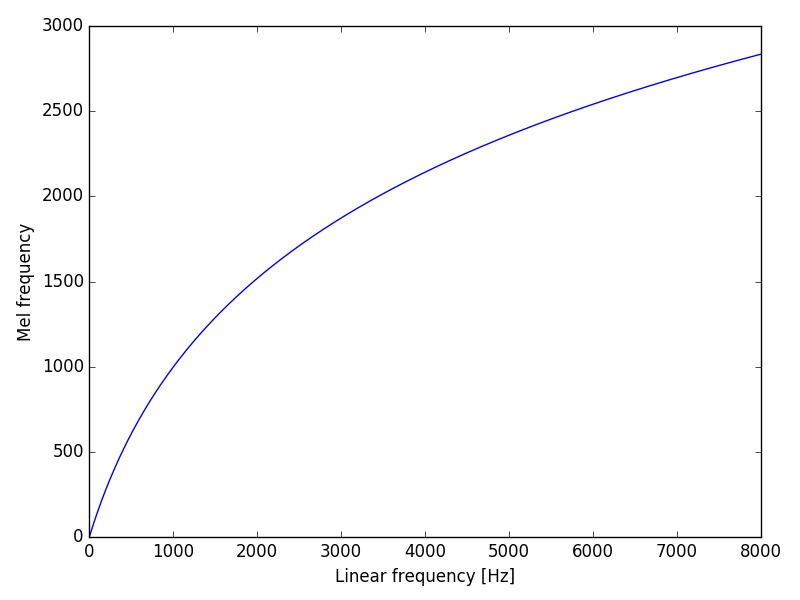
\includegraphics[width=0.7\linewidth]{images/MFCC_mel_to_linear}
		\caption{Relation between mel and linear frequency}
		\label{fig:MFCC_mel_to_linear}
	\end{figure}
	
	In order to convert a signal frame into mel scale it is necessary to prepare mel filter bank. The relation between mel and linear scale is shown in figure \ref{fig:MFCC_mel_to_linear}. Firstly, one must find mel representation of selected frequency boundaries according to following equation:
	
	\begin{equation}
		m(f) = 1127 \ln\left(1 + \frac{f}{700}\right)
	\end{equation}
	
	In this case it would be:
	
	\begin{itemize}
		\item $m_l = m(f_l) = 23.89$
		\item $m_h = m(f_h) = 2146.08$
	\end{itemize}
	
	After that it is necessary, to calculate \gls{n_c} + 2 equally spaced mel values from range \mbox{(\gls{m_l}, \gls{m_h})}. They are expressed by following equation:
	
	\begin{equation}
		m_n = m_l + n \cdot \frac{(m_h - m_l)}{n_c + 1}
	\end{equation}
	
	This results with following array:
	
	\begin{verbatim}
	m_n =  [0023.89	0102.49	0181.09	0259.69	0338.29	0416.89	0495.49	0574.09	0652.69	0731.29	0809.89	0888.49	0967.09	1045.69	1124.28	1202.88	1281.48	1360.08	1438.68	1517.28	1595.88	1674.48	1753.08	1831.68	1910.28	1988.88	2067.48	2146.08]
	\end{verbatim}
	
	It is now necessary to switch back into frequency domain, using equation:
	
	\begin{equation}
		f(m) = 700 \left(e^{m/1127} - 1 \right)
	\end{equation}
	
	This results with obtaining logarithmic spaced frequency array, with boundaries the same as initially picked:
	
	\begin{verbatim}
	f_n =  [0015.00	0066.65	0122.02	0181.40	0245.06	0313.33	0386.52	0465.00	0549.15	0639.38	0736.12	0839.86	0951.08	1070.34	1198.22	1335.33	1482.35	1639.98	1809.00	1990.23	2184.55	2392.90	2616.31	2855.85	3112.70	3388.09	3683.38	4000.00]	
	\end{verbatim}
	
	Having this frequency array lets to produce mel filters. Each filter ($F_k$) is an array of \gls{N_frame} elements, where \gls{N_frame} is the length of the frame. Filters are indexed by range [1,\gls{n_c}]. Value of each element of a filter is defined by following equation:
	
	\begin{equation}
	F_k(n) = \begin{dcases}
				0, n < f_{k-1} \\
				\frac{n - f_{k-1}}{f_k - f_{k-1}}, f_{k-1} \leq n \leq f_k \\
				\frac{f_{k+1} - n}{f_{k+1} - f_k}, f_k \leq n \leq f_{k+1} \\
				0, n > f_{k+1}					
			 \end{dcases}
	\end{equation}
	
	Example filter bank can be seen in figure \ref{fig:MFCC_filter_bank}. It is easy to notice that each mel filter is simply passing some part of signal spectrum.
	
	\begin{figure} [!th]
		\centering
		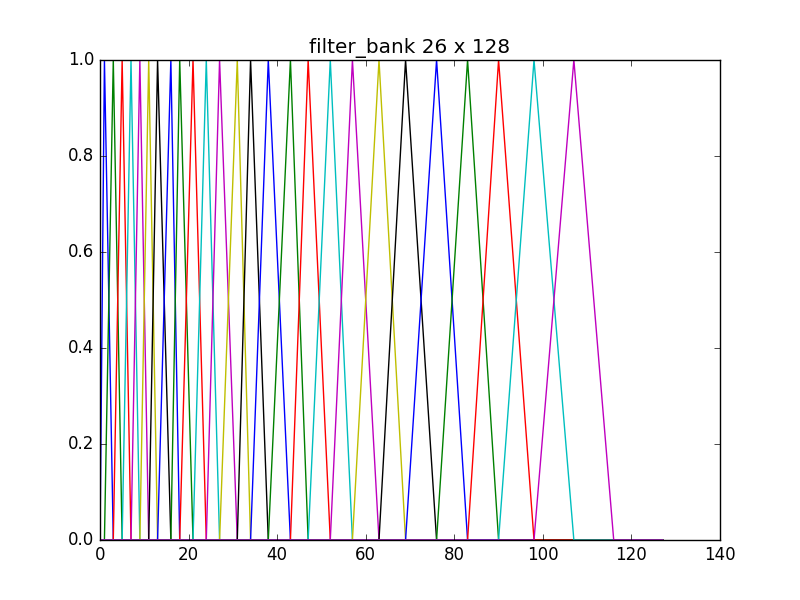
\includegraphics[width=0.7\linewidth]{images/MFCC_filter_bank}
		\caption{Example filter bank}
		\label{fig:MFCC_filter_bank}
	\end{figure}

	Having filter bank prepared, one should simply apply each filter on previously calculated frame spectrum. This operation can be described by following equation:
	
	\begin{equation}
		S_k(n) = S(n) \cdot F_k(n)
	\end{equation}
	
	where:
	
	\begin{itemize}
		\item $S_k(n)$ -- current frame filtered with k-th mel filter
		\item $S(n)$ -- current frame in frequency domain
		\item $F_k(n)$ -- k-th mel filter
	\end{itemize}
	
	Having \gls{n_c} filtering result, it is necessary to calculate logarithmic power of each result in the following way:
	
	\begin{equation} \label{eq:mfcc_sumation}
		MFCC_k = \ln \left( \varepsilon_f + \sqrt{\sum_{n=0}^{N_{frame}} |S_k(n)|^2} \right)
	\end{equation}
	
	Addition of \gls{epsilon} is necessary in order to prevent numerical errors if sum from equation \ref{eq:mfcc_sumation} would be equal to 0. The procedure ends with extracting \gls{n_c} \gls{MFCC} from each frame.
	
	\subsection{Applying Discrete Cosine Transform}
	
	The last step that requires doing is to switch back into time domain. In theory this could be done by inverse \gls{FFT} algorithm, but this would again result with result in complex numbers. Therefore it is better to use Discrete Cosine Transform \gls{DCT}. Functionally this operation is analogous to Fourier Transform, except for the fact that it is defined for real numbers.
	
	\subsection{Liftering} \label{sec:liftering}
	
	One of the properties of \gls{MFCC} is that their variance and the average numerical value are decreasing with increase of their index. It basically means that only some subsequence of already calculated $MFCC_k$ array should be taken for further processing. Another \gls{MFCC} property is that the first coefficient is proportional to the mean of the log spectral energy channels and indicates overall lever for the speech frame. It means that information held by first coefficient is too generous to be used for speaker recognition \cite{SpeechAnalysis}. \\
	
	Because of following properties of \gls{MFCC}, one should define another parameter of feature extraction process -- \gls{n_l} -- this is number of \gls{MFCC} used for further processing. This steps results with construction of \gls{V_n}, which is vector of extracted speaker features in particular frame, where:
	
	\begin{equation}
		\forall_{n \in [1, n_l]} V_n = MFCC_{n+1}
	\end{equation}	 
	
	\subsection{Vector enhancements}
	
	The result of liftering is vector \gls{V_n} and practically it contains all of the features of the speaker. Although the accuracy of classification algorithms described in section \ref{sec:classification} can be enhanced by some further processing of feature vector. Such actions are common in data mining techniques and usually they do not depend on kind of processed data.
	
	\subsubsection{Appending deltas}
	
	Previously described \gls{MFCC} extraction assumed that all of the cepstral coefficients are stationary, although while analysis of speaker signal it is also relevant to take into consideration speed and acceleration of pronounced vowels \cite{SpeechAnalysis}. The popular algorithm for approximating these dynamic parameters is linear regression. The $n$-th dynamic coefficient of order $K$ of current frame can be evaluated in the following way:
	
	\begin{equation}
		\delta^K_n = \frac{\sum_{k=-K}^{K} k \cdot (V_{n+k} - V_{n-k})}{2 \sum_{k=-K}^{K} k^2}
	\end{equation}
	
	Such calculated deltas of order 1 and 2 are then appended to feature vector as presented:
	
	\begin{equation}
		\tilde{V} = [V_1 \; V_2 \; ... \; V_{n_l} \quad \delta^1_1 \; \delta^1_2 \; ... \; \delta^1_{n_l} \quad \delta^2_1 \; \delta^2_2 \; ... \; \delta^2_{n_l}]^T
	\end{equation}
	
	\subsubsection{Cepstral mean subtraction}
	
	One of difficulties during classifying incoming samples is changing channel influence on received signal. One of possibilities of compensating it is Cepstral Mean Subtraction \gls{CMS} algorithm \cite{CepstralMeans}. There are many approaches of calculating it and the most straightforward method looks as follows:
	
	\begin{equation}
		\forall_{n \in [1, 3 \cdot n_l]} \forall_{k \in [1,N_{frames}]} \mathrm{A}_{n,k} = \mathrm{A}_{n,k} - \frac{1}{N_{frames}} \sum_{l=1}^{N_{frames}} \mathrm{A}_{n,l}
	\end{equation}
	
	where:
	
	\begin{itemize}
		\item $\mathrm{A}$ -- matrix of coefficients of whole processed sample.
	\end{itemize}
	
	\subsubsection{Feature warping}
	
	The last step of parametrization used in this thesis is feature warping. This operation lets to reduce impact of the channel properties on incoming stream of data and makes it also more independent of additive noise \cite{FeatureWarping}. Feature warping is simply nonlinear conversion of distribution of every extracted coefficient independently that is supposed to make it similar to normal distribution. In order to do so one has to proceed following steps:
	
	\begin{enumerate}
		\item Get single row ($r$) of extracted coefficients,
		\item Find minimum and maximum of $r$ -- it lets to calculate $\mu$ and $\sigma$ values of desired normal distribution, according to following equation:
		\begin{equation}
			\mu = \frac{\min r + \max r}{2}
		\end{equation}
		\begin{equation}
			\sigma = \frac{\max r - \min r}{6}
		\end{equation}
		\item Calculate Cumulative Distribution Function of chosen normal distribution ($p$). Example of such \gls{CDF} is shown in figure \ref{fig:feature_warping_norm_cdf},
		
		\begin{figure}[!th]
			\centering
			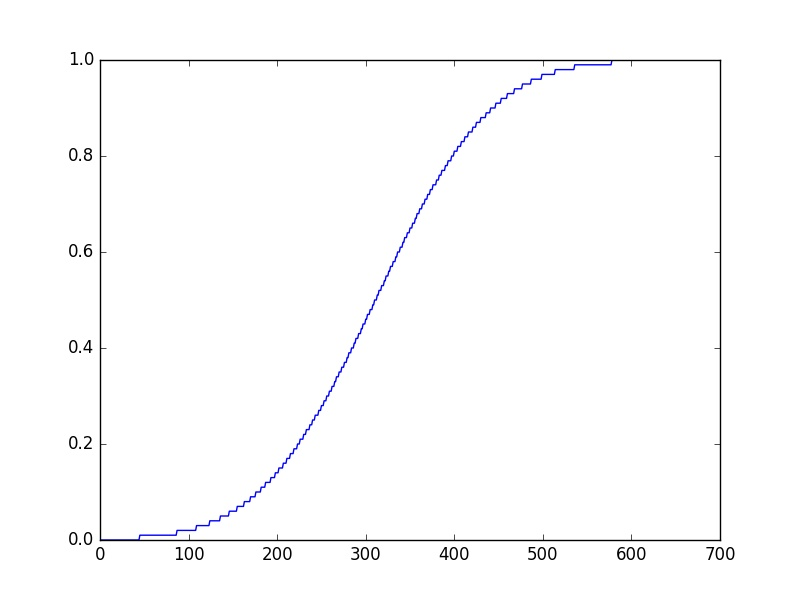
\includegraphics[width=0.7\linewidth]{images/feature_warping_norm_cdf}
			\caption{Example of \gls{CDF} of normal distribution}
			\label{fig:feature_warping_norm_cdf}
		\end{figure}
		
		\item Calculate \gls{CDF} of $r$ ($q$)-- example shown in figure \ref{fig:feature_warping_noised_cdf},

		\begin{figure}[!th]
			\centering
			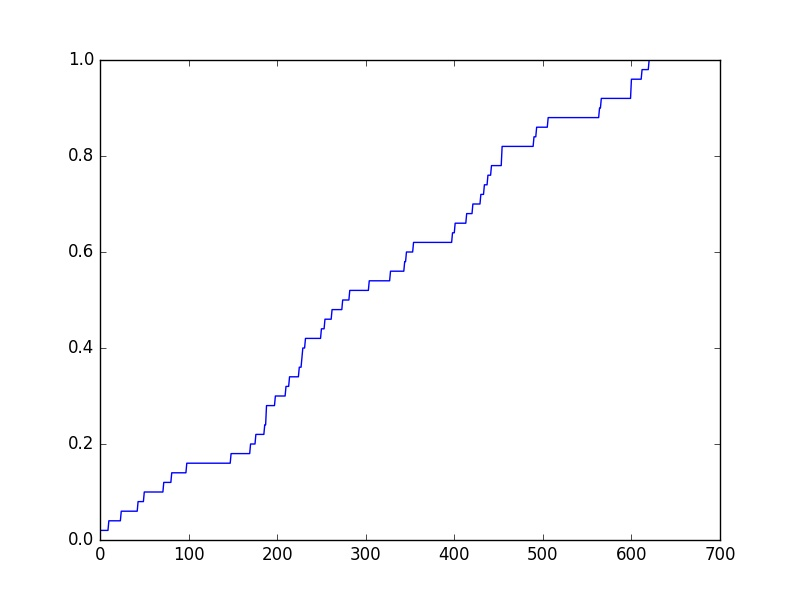
\includegraphics[width=0.7\linewidth]{images/feature_warping_noised_cdf}
			\caption{\gls{CDF} of noised signal}
			\label{fig:feature_warping_noised_cdf}
		\end{figure}

		\item Prepare remapping table for vector $r$. Table would indicate that each $\alpha$ value should be substituted with $\beta$, where $\beta$ can be calculated from following equation \cite{feature_warping_description}:
		
		\begin{equation} \label{eq:feature_warping}
			q(\alpha) = p(\beta)
		\end{equation}
		
		\item Remap $r$ with prepared table -- example showin in figure \ref{fig:feature_warping_featured_cdf}.
		
		\begin{figure}[!th]
			\centering
			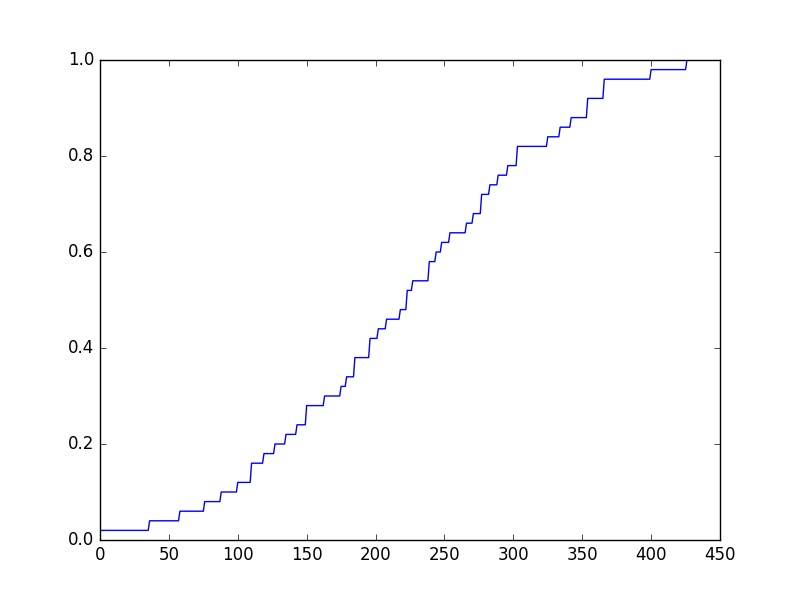
\includegraphics[width=0.7\linewidth]{images/feature_warping_featured_cdf}
			\caption{\gls{CDF} of noised signal after feature warping}
			\label{fig:feature_warping_featured_cdf}
		\end{figure}
	\end{enumerate}
	
	As previously mentioned this method lets to remove additive noise and undesired properties of channel from extracted signal. The effectiveness of feature warping can be seen in figure \ref{fig:feature_warping_summary}, where an output of feature warping of initial signal and its distortion is very similar .
	
	\begin{figure}[!th]
		\centering
		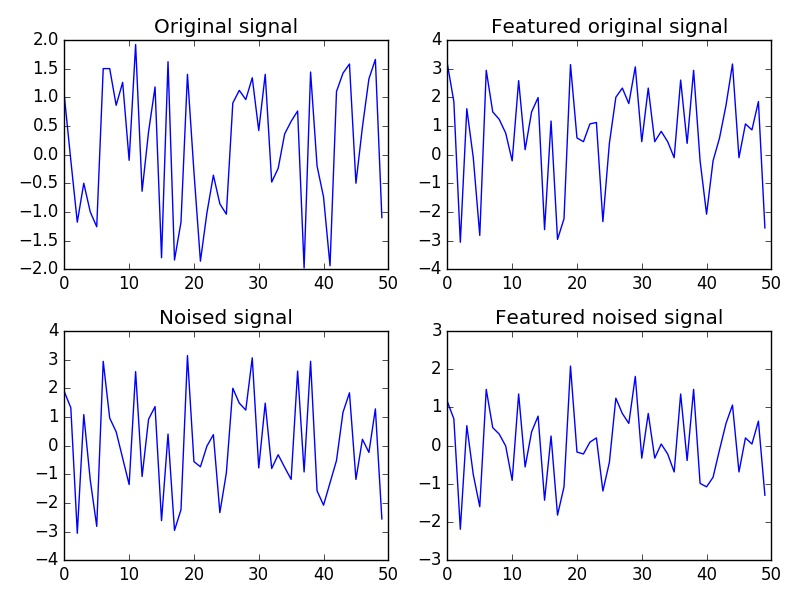
\includegraphics[width=0.7\linewidth]{images/feature_warping_summary}
		\caption{Summary of feature warping effectiveness}
		\label{fig:feature_warping_summary}
	\end{figure}

	\FloatBarrier
	
	\section{Classification} \label{sec:classification}
	
	The general goal of classification methods is to extract the only necessary information of incoming samples and to collect them as set of coefficients that would let to classify other samples properly. Problem defined in this thesis is Binary Classification \cite{IntroductionToMachineLearning}. One can find many techniques used to solve such problem and some of them will be described in this section.
	
	\subsection{Popular classification techniques}
	
	\subsubsection{Gaussian Mixtures}
	
	The general assumption of speaker model during Gaussian Mixtures Modeling is that it composes of several states and the observed output is the result of hidden (impossible to be directly measured) state. Distribution of the output for specific $i$-th state is given by following equation:
	
	\begin{equation} \label{eq:gaussian_pdf}
		b_i(x) = \frac{1}{(2 \pi)^{D/2} |\Sigma_i|^{1/2}} \times exp \left[ - \frac{1}{2} (x - \mu_i)^T (\Sigma_i)^{-1} (x - \mu_i) \right]
	\end{equation}
	
	where:
	
	\begin{itemize}
		\item $D$ -- number of dimensions of measured features,
		\item $\mu_i$ -- the state mean vector,
		\item $\Sigma_i$ -- the state covariance matrix.
	\end{itemize}
	
	Function $b_i$ can be interpreted as multidimensional Gaussian probability density function. It basically means that for some fixed state of researched model observed vectors would fall into Gaussian distribution (accordingly to number of dimensions of extracted features). Such assumption leads to following \gls{GMM} equation:
	
	\begin{equation} \label{eq:gmm_probability}
		p(x|\lambda) = \sum_{i=1}^{M} p_i b_i(x)
	\end{equation}
	
	where:
	
	\begin{itemize}
		\item $\forall_{i \in [1, M]} \ \lambda = (p_i, \mu_i, \Sigma_i)$ -- certain reference model parameters,
		\item $p_i$ -- probability of occurring specific state for reference model.
	\end{itemize}
	
	Equation \ref{eq:gmm_probability} can be interpreted in the following way: \emph{The probability that received sample $x$ came from reference model $\lambda$ is equal to sum of the probabilities that $x$ was generated by $\lambda$ in state $i$ multiplied by probability of occurrence of state $i$}. \\
	
	In speaker recognition analysis the state can be interpreted as specific sound generated by a speaker (like vowel). The probabilities $p_i$ are more bounded to text dependent information, thus they are considered to be equal to each other. The task of \gls{GMM} algorithm is to define number of states and to find model parameters $\lambda$. They are obtained in unsupervised manner by using the expectation-maximization algorithm (EM) \cite{GaussianMixtures}.
	
	\subsubsection{Principal Component Analysis}
	
	\gls{PCA} is an algorithm that lets to reduce number of dimensions of extracted feature vectors. It basically tries to transform the basis of received vectors into another that would better express given data set. It serves to remove redundancy of information and its output is used as an input for algorithms like previously described \gls{GMM}. The \gls{PCA} assumes:
	
	\begin{itemize}
		\item linearity of processed data,
		\item orthonormality of vectors of original basis.
	\end{itemize}
	
	\gls{PCA} is trying to find matrix $\mathrm{P}$ that would transform original basis $\mathrm{X}$ into $\mathrm{Y}$ according to following equation:
	
	\begin{equation}
		\mathrm{P} \mathrm{X} = \mathrm{Y}
	\end{equation}
	
	in such a way that data transformed into new basis would better express searched properties. The measure of quality of obtained new properties is the covariance between them. The covariance equal to 0 indicates no correlation between properties, i.e., good representation of processed properties. Therefore covariance matrix $\mathrm{S}_\mathrm{X}$ is extracted of processed data and coefficients of matrix $\mathrm{P}$ are picked in such a way that $\mathrm{Y}$ would be as close to diagonal matrix as its possible. \\
	
	It is only necessary to assume specific number of properties to be extracted of given data and this should be chosen carefully according to exact classification problem \cite{PCA_tutorial}.
	
	\subsubsection{Neural networks}

	Neural network is a concept that basis on this, how human brain works. It consists of neurons and each neuron has several inputs and only one output. Its mathematical model is shown in figure \ref{fig:neruon_model}.
	
	\begin{figure} [!th]
		\centering
		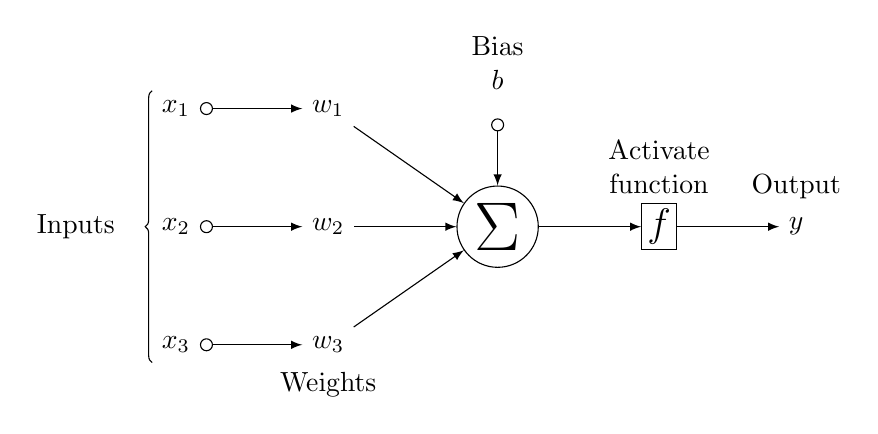
\begin{tikzpicture}[
		init/.style={
			draw,
			circle,
			inner sep=2pt,
			font=\Huge,
			join = by -latex
		},
		squa/.style={
			draw,
			inner sep=2pt,
			font=\Large,
			join = by -latex
		},
		start chain=2,node distance=13mm
		]
		\node[on chain=2] 
		(x2) {$x_2$};
		\node[on chain=2,join=by o-latex] 
		{$w_2$};
		\node[on chain=2,init] (sigma) 
		{$\displaystyle\Sigma$};
		\node[on chain=2,squa,label=above:{\parbox{2cm}{\centering Activate \\ function}}]   
		{$f$};
		\node[on chain=2,label=above:Output,join=by -latex] 
		{$y$};
		\begin{scope}[start chain=1]
		\node[on chain=1] at (0,1.5cm) 
		(x1) {$x_1$};
		\node[on chain=1,join=by o-latex] 
		(w1) {$w_1$};
		\end{scope}
		\begin{scope}[start chain=3]
		\node[on chain=3] at (0,-1.5cm) 
		(x3) {$x_3$};
		\node[on chain=3,label=below:Weights,join=by o-latex] 
		(w3) {$w_3$};
		\end{scope}
		\node[label=above:\parbox{2cm}{\centering Bias \\ $b$}] at (sigma|-w1) (b) {};
		
		\draw[-latex] (w1) -- (sigma);
		\draw[-latex] (w3) -- (sigma);
		\draw[o-latex] (b) -- (sigma);
		
		\draw[decorate,decoration={brace,mirror}] (x1.north west) -- node[left=10pt] {Inputs} (x3.south west);
		\end{tikzpicture}
		\caption{Neuron model \cite{neural_network_diagrams}}
		\label{fig:neruon_model}
	\end{figure}
	
	The equation computed by neuron that has $N $ inputs is the following:
	
	\begin{equation}
		y = f(b + \sum_{i=1}^{N} x_i \cdot w_i)
	\end{equation}
	
	where:
	
	\begin{itemize}
		\item $f: (-\infty, \infty) \mapsto [-1, 1]$ -- activate function,
		\item $b$ -- bias of the neuron,
		\item $w_i$ -- weights of the neuron,
		\item $x_i$ -- incoming input.
	\end{itemize}
	
	Usually in single neural network all of the neurons share the same activate function. Typical examples of such functions are shown in figure \ref{fig:activate_functions}. \\
	
	\begin{figure}
		\centering
		\begin{subfigure}{.33\textwidth}
			\centering
			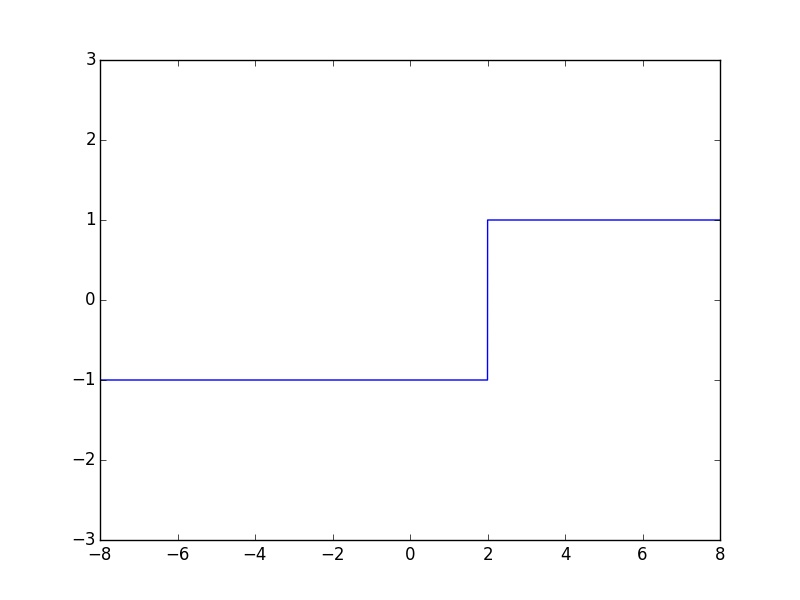
\includegraphics[width=.8\linewidth]{images/act_func_threshold}
			\caption{threshold}
		\end{subfigure}%
		\begin{subfigure}{.33\textwidth}
			\centering
			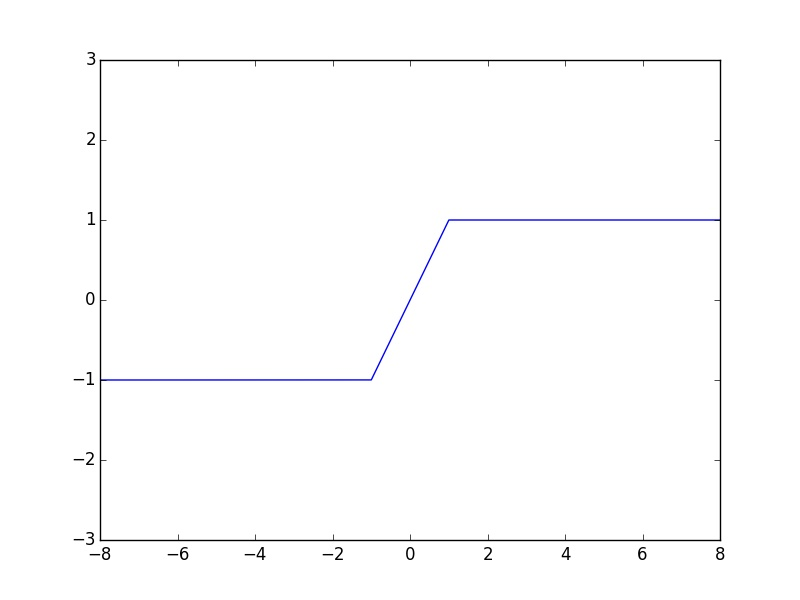
\includegraphics[width=.8\linewidth]{images/act_func_piecewise_lin}
			\caption{piecewise linear}
		\end{subfigure}
		\begin{subfigure}{.33\textwidth}
			\centering
			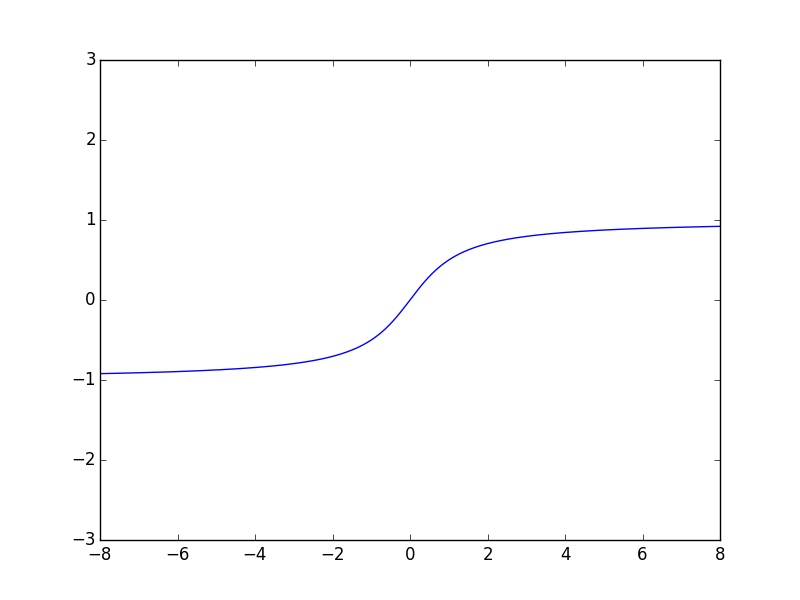
\includegraphics[width=.8\linewidth]{images/act_func_atan}
			\caption{scaled arctangent}
		\end{subfigure}
		\caption{Example activate functions}
		\label{fig:activate_functions}
	\end{figure}
	
	Neurons are connected in a network according to chosen architecture. The choice of architecture depends on the nature of the problem. In authentication problem the number of inputs could be equal to the quantity of dimensions of feature vector and the output could be only one number (authentication successful or failed). The number and size of hidden layers could be chosen in an experimental way. Example neural network architecture is shown in figure \ref{fig:neural_network_architecture}. \\
	
	\begin{figure} [!th]
		\centering
			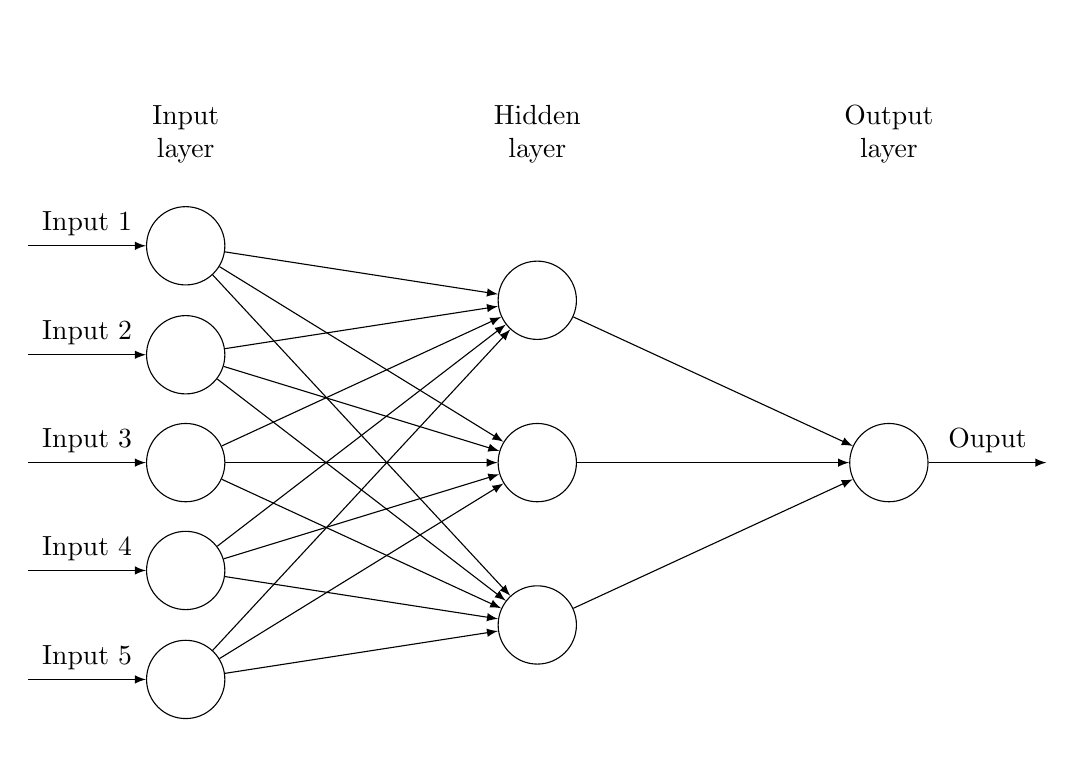
\begin{tikzpicture}[
			plain/.style={
				draw=none,
				fill=none,
			},
			net/.style={
				matrix of nodes,
				nodes={
					draw,
					circle,
					inner sep=10pt
				},
				nodes in empty cells,
				column sep=2cm,
				row sep=-9pt
			},
			>=latex
			]
			\matrix[net] (mat)
			{
				|[plain]| \parbox{1.3cm}{\centering Input\\layer} & |[plain]| \parbox{1.3cm}{\centering Hidden\\layer} & |[plain]| \parbox{1.3cm}{\centering Output\\layer} \\
				& |[plain]| \\
				|[plain]| & \\
				& |[plain]| \\
				|[plain]| & |[plain]| \\
				& & \\
				|[plain]| & |[plain]| \\
				& |[plain]| \\
				|[plain]| & \\
				& |[plain]| \\
			};
			\foreach \ai [count=\mi ]in {2,4,...,10}
			\draw[<-] (mat-\ai-1) -- node[above] {Input \mi} +(-2cm,0);
			\foreach \ai in {2,4,...,10}
			{\foreach \aii in {3,6,9}
				\draw[->] (mat-\ai-1) -- (mat-\aii-2);
			}
			\foreach \ai in {3,6,9}
			\draw[->] (mat-\ai-2) -- (mat-6-3);
			\draw[->] (mat-6-3) -- node[above] {Ouput} +(2cm,0);
			\end{tikzpicture}
			\caption{Example neural network architecture \cite{neural_network_diagrams}}
			\label{fig:neural_network_architecture}
	\end{figure}
	
	The process of learning neural network is supposed to find such set of neurons coefficients that would force the network to give proper results according to reference data \cite{neural_networks_tutorial}.
	
	\subsubsection{Support Vector Machine}
	
	In \gls{SVM} the learning data is assumed to consist of pairs $(x_i, y_i)$, where:
	
	\begin{itemize}
		\item $x_i$ -- data point,
		\item $y_i$ -- predicted result of classification (1 if point belongs to specific class and -1 when its not).
	\end{itemize}
	
	\gls{SVM} is a classification method that is focused on finding such a hyperplane that would hold specific relation with learning points. In general chosen hyperplane would be defined by two vectors $w$ and $b$ and all of its points $x$ would have to hold the following equation:
	
	\begin{equation}
		w^T x + b = 0			
	\end{equation}
	
	Having these vectors lets to construct the following classifier:
	
	\begin{equation}
		h_{w,b}(x) = g(w^T x + b)
	\end{equation}
	
	where:
	
	\begin{equation}
		g(x) = 
		\begin{dcases}
			1, x \geq 0 \\
			-1, x < 0
		\end{dcases}
	\end{equation}
	
	During learning process (finding vectors $w$ and $b$) one defines \emph{functional margin} as:
	
	\begin{equation}
		\gamma_i = y_i (w^T x_i + b)
	\end{equation}
	
	It is worth to notice that $\gamma_i$ can be interpreted as measure of confidence for specific point, because the greater $\gamma_i$ is, the more distant of chosen hyperplane point $x_i$ is. Moreover if $\gamma_i$ is positive, then $h_{w,b}(x_i) = y_i$ -- which means that point $x_i$ is classified properly. \\
	
	Although scaling $w$ and $b$ by the same positive constant would also increase $\gamma_i$ without any significant correction of chosen parameters. That is why it is comfortable to assume that \mbox{$||w|| = 1$}. In such case $\gamma_i$ would be a reliable measure of quality of chosen vectors $w$ and $b$. Since data set consists of $N$ samples, the overall functional margin is defined as:
	
	\begin{equation}
		\gamma = \min_{i \in [1,N]} \gamma_i
	\end{equation}
	
	It leads to conclusion that \gls{SVM} algorithm during learning process is trying to determine values of vectors $w$ and $b$ in such a way that they would maximize overall functional \mbox{margin $\gamma$ \cite{SVM_tutorial}}.

	\subsection{Synergy of classification techniques}
	
	In many real systems several classification techniques are used simultaneously for interpreting the same results and their outputs (like logarithmic probability) are then combined in some way. \\
	
	The simplest solution of interpreting such probability would be comparing it with some threshold chosen during learning phase. Thanks to having many samples and many techniques, this approach could be extended by using weighted/moving average of probabilities between different classifiers. Results of simple classification algorithm are also shown in section \ref{sec:example_classification}.
	
	\subsection{Example classification results} \label{sec:example_classification}
	
	Figure \ref{fig:raw_sets_of_data} is showing some random data of 2 classes. The algorithm applied to process this data was \gls{GMM} (number of states of reference model was set to 3). Two classifier were used:
	
	\begin{itemize}
		\item one used to fit to first set of data,
		\item second used to fit to second set of data.
	\end{itemize}
	
	\begin{figure}[!th]
		\begin{subfigure}{.5\textwidth}
			\centering
			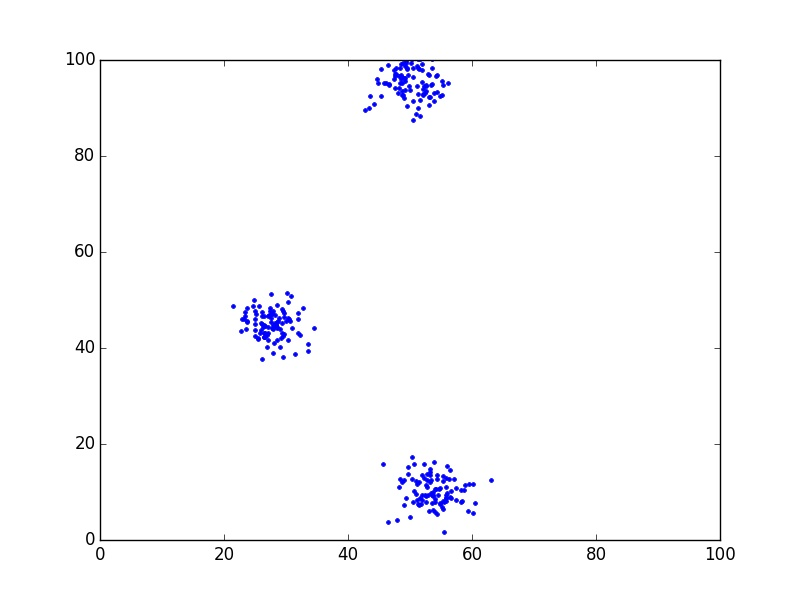
\includegraphics[width=.8\linewidth]{images/gmm_raw_data_1}
			\caption{class 1}
		\end{subfigure}%
		\begin{subfigure}{.5\textwidth}
			\centering
			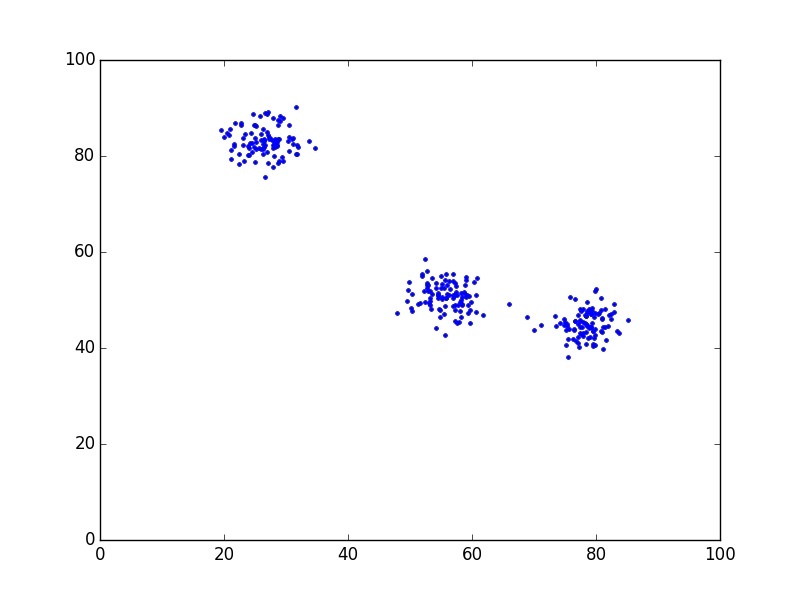
\includegraphics[width=0.8\linewidth]{images/gmm_raw_data_2}
			\caption{class 2}
		\end{subfigure}
		\caption{Sets of data}
		\label{fig:raw_sets_of_data}
	\end{figure}
	After fitting process both sets were applied to first trained classifier. Figure \ref{fig:gmm_score_comp} shows logarithmic probability of belonging to set for both sets. It can be easily noticed that class 1 reaches much higher score then class 2. It lets to choose a threshold of defining sample as belonging or not belonging to specific class. The threshold chosen in this case was $-15$. Then it was possible to construct classifier that would distinguish three kinds of samples:
	
	\begin{itemize}
		\item belonging to class 1,
		\item belonging to class 2,
		\item unassigned points.
	\end{itemize}
	
	An algorithm used to distinguish samples is following:
	
	\begin{equation}
		\mathcal{A}(x) = \begin{dcases}
		\mathrm{CLASS\_1}, \quad   \mathrm{GMM}_1.\mathrm{score}(x) \geq -15 \\
		\mathrm{CLASS\_2}, \quad   \mathrm{GMM_2.score(x)} \geq -15 \  \land \ \mathrm{GMM}_1.\mathrm{score}(x) < -15\\
		UNASSIGNED, \quad otherwise \\
		\end{dcases}	
	\end{equation}
	
	\begin{figure}
		\centering
		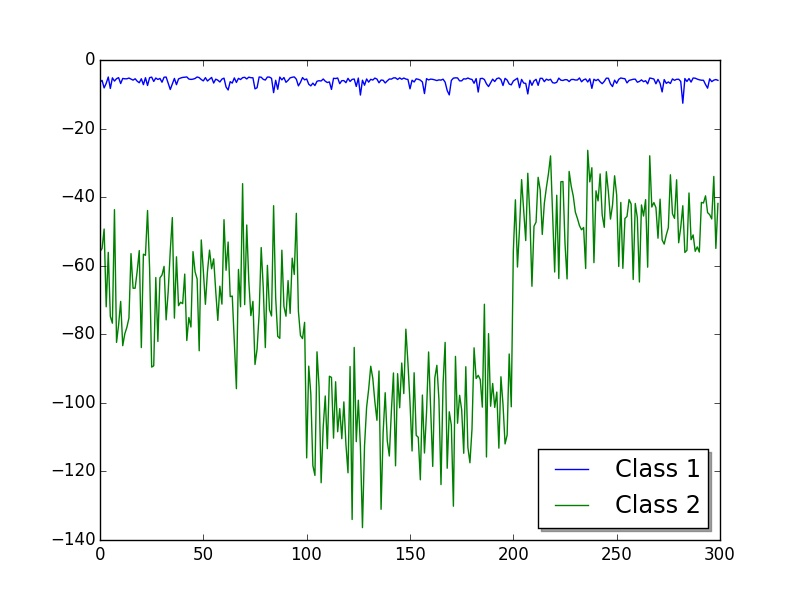
\includegraphics[width=0.6\linewidth]{images/gmm_score_comp}
		\caption{Comparing of scores of datas belonging to two classes}
		\label{fig:gmm_score_comp}
	\end{figure}

	Described algorithm $\mathcal{A}$ was applied to random set of data. Results of used classification are shown in figure \ref{fig:gmm_classified}. Where:
	
	\begin{itemize}
		\item blue dots -- samples initially belonging to class 1,
		\item red dots -- samples initially belonging to class 2,
		\item cyan dots -- samples of random set assigned to class 1,
		\item magenta dots -- samples of random set assigned to class 2,
		\item green dots -- unassigned samples.
	\end{itemize}
	
	\begin{figure}
		\centering
		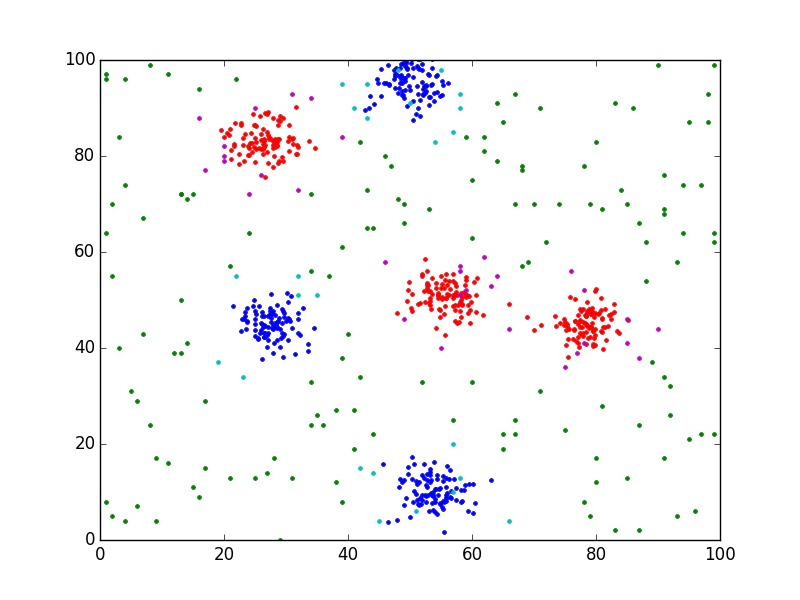
\includegraphics[width=0.6\linewidth]{images/gmm_classified}
		\caption{Classified data}
		\label{fig:gmm_classified}
	\end{figure}

	
	\chapter{Implementation description}
	
	Voice authorization mechanism described in chapter \ref{ch:speaker_recognition} was implemented in \texttt{Python 2.7} language. It generally consists of two logical parts:
	
	\begin{itemize}
		\item processing -- it consists of all of the mathematical operations executed on incoming samples,
		\item interface -- all classes defined in processing could be used separately and imported in different projects, but GUI interface is a simple wrapper that lets to use full functionality of presented library without necessity of writing any code. Since it is not focused on theoretical aspect of speaker recognition it will not be covered in this thesis.
	\end{itemize}
	
	\section{Library configuration}
	
	In order to make configuration of the library easy and interface independent it is mostly done by json file (called \texttt{.config} by default). The example \texttt{.config} is shown in listing \ref{lst:.config}.\\
	
	\begingroup
	\captionof{listing}{Example \texttt{.config} file \label{lst:.config}}
	\inputminted[linenos=true]{json}{../automatic_speaker_recognition/.config}
	\endgroup
	
	\section{Helper classes}
	
	\subsection{Constants}
	
	Non processing parameters of the library (like file paths and file patterns) are defined in this class. It lets to easily distinguish algorithmic configuration from environmental one.
	
	\subsection{Wave processor}
	
	Only one method of this class is used by other classes. It is called \texttt{extract\_raw\_data} and its task is to decode \gls{WAV} file into plain array of numbers.
	
	\subsection{Mel filter bank}
	
	This class is supposed to help during mel filtering phase. In its constructor it prepares array of filters. Its only function used publicly after creation of an object is \texttt{filter\_data} and its body is presented in listing \ref{lst:filter_data}.\\
	
	\begingroup
	\captionof{listing}{Body of \texttt{filter\_data} function \label{lst:filter_data}}
	\begin{minted}[linenos=true]{python}	
def filter_data(self, data):
    res = []	
    for mel_filter in self.filters:
    arr = zip(mel_filter, data)
    res.append([mel_coeff * data_el for (mel_coeff, data_el) in arr])	
return res	
	\end{minted}
	\endgroup
	\vspace{1em}
	
	It is easy to notice that this function simply gets input array of size $N$ and then filters it with every filter in its bank, resulting with matrix of size $N \times M$ on output, where:
	
	\begin{itemize}
		\item $N$ -- number of data samples,
		\item $M$ -- number of used filters.
	\end{itemize}
	
	\subsection{Data dumper}
	
	This is a class that is used for all of the operations that should load/store data of any kind (except for \gls{WAV} files). It is also used to store samples of processing steps as plots that could help to analyze it. The interface of this class consists of following functions:
	
	\begin{itemize}
		\item \texttt{store\_json\_data} -- writes given data into specified json file
		\item \texttt{load\_json\_data} -- loads and returns data from the specified json file
		\item \texttt{store\_binary\_data} -- writes given data into specified binary file
		\item \texttt{load\_binary\_data} -- loads and returns data from the specified binary file
		\item \texttt{dump\_plot} -- stores given data as a specified kind of plot. Supported plot modes are the following:
		\begin{itemize}
			\item \texttt{dim\_2\_plot} -- simple plot of one dimensional array,
			\item \texttt{dim\_2\_plot\_mult} -- multiple plot of arbitrary number of arrays given as an argument,
			\item \texttt{dim\_3\_plot} -- 3 dimensional plot of 2 dimensional array, where 3rd dimension is expressed by color,
			\item \texttt{dim\_2\_rect} -- bar graph.
			
		\end{itemize}
	\end{itemize}
	
	\section{Signal parametrizer}
	
	The full implementation of this class can be found in appendix \ref{ch:impl_signal_param}. Its only publicly used method is \texttt{extract\_mfcc} and it will be covered in details in this section.\\
	
	\begingroup
	\captionof{listing}{Preemphase \label{lst:preemphase}}
	\begin{minted}[linenos=true]{python}
if self.dump_options['dumps_enabled']:
    DataDumper.dump_plot(data, 'original_signal', 'dim_2_plot')

if self.log_callback is not None:
    self.log_callback.set('{:40} pre_emphase'.format(filename))
	
data = self.pre_emphase(data)

if self.dump_options['dumps_enabled']:
    DataDumper.dump_plot(data, 'preemphased_signal', 'dim_2_plot')
	\end{minted}
	\endgroup
	\vspace{1em}
	
	Listing \ref{lst:preemphase} shows the first step of \gls{MFCC} extraction, which is preemphase. Lines 1-2,9-10 are used for dumping processing results of each stage and lines 4-5 are setting log callback that is used by GUI (in order to inform user of the program about every step of application). These lines are not bounded to extraction algorithm and can be ignored by proper configuration provided in $.config$ file.\\
	
	\begingroup
	\captionof{listing}{Decimation and dividing into frames \label{lst:decimation_divide}}
	\begin{minted}[linenos=true]{python}
if self.log_callback is not None:
self.log_callback.set('{:40} decimate'.format(filename))
data = self.decimate(data)

if self.log_callback is not None:
self.log_callback.set('{:40} divide_into_frames'.format(filename))
frames = self.divide_into_frames(data)
	\end{minted}
	\endgroup
	\vspace{1em}
		
	Listing \ref{lst:decimation_divide} shows another two steps of \gls{MFCC} extraction which is decimating incoming data and dividing it into frames. Decimation is used for optimization reasons. It lets to significantly reduce calculation complexity without loss of quality of results.\\
	
	\begingroup
	\captionof{listing}{Frame processing \label{lst:frame_processing}}
	\begin{minted}[linenos=true]{python}
res = []

for ind, frame in enumerate(frames):

    if self.log_callback is not None:
        self.log_callback.set('{:40} processing {} of {} frames'
                         .format(filename, ind, len(frames)))
    
    frame = self.zero_pad(frame)

    if self.dump_options['dumps_enabled'] and ind == \
       self.dump_options['selected_frame']:
        DataDumper.dump_plot(frame, 'padded_signal', 'dim_2_plot')

    if self.steps['perform_windowing']:
        frame = self.apply_windowing(frame)

    if self.dump_options['dumps_enabled'] and ind == \
       self.dump_options['selected_frame']:
        DataDumper.dump_plot(frame, 'windowed_signal', 'dim_2_plot')

    frame = self.apply_fft(frame)

    if self.dump_options['dumps_enabled'] and ind == \
       self.dump_options['selected_frame']:
        DataDumper.dump_plot(frame, 'after_fft_signal', 'dim_2_plot')

    mel_filter_results = self.mel_filter_bank.filter_data(frame)
    vector = []

    if self.dump_options['dumps_enabled'] and ind == \
    self.dump_options['selected_frame']:
        DataDumper.dump_plot(mel_filter_results,
                             'mel_filtered_signal',
                             'dim_3_plot')

    for mel_filter_result in mel_filter_results:
        power = self.calculate_signal_power(mel_filter_result)
        vector.append(math.log(power))

    if self.dump_options['dumps_enabled'] and ind == \
       self.dump_options['selected_frame']:
        DataDumper.dump_plot(vector, 'mel_power_signal', 'dim_2_rect')

    vector = self.discrete_cosine_transform(vector)

    if self.dump_options['dumps_enabled'] and ind == \
       self.dump_options['selected_frame']:
        DataDumper.dump_plot(vector,
                             'cosine_transformed_signal',
                             'dim_2_rect')

    vector = self.liftering(vector)

    if self.dump_options['dumps_enabled'] and ind == \
       self.dump_options['selected_frame']:
        DataDumper.dump_plot(vector, 'liftered_signal', 'dim_2_rect')

    res.append(vector)

if self.dump_options['dumps_enabled']:
    DataDumper.dump_plot(res, 'parametrized_raw', 'dim_3_plot')
	\end{minted}
	\endgroup
	\vspace{1em}
		
	Listing \ref{lst:frame_processing} is showing steps executed on each processed frame. These are:
	
	\begin{itemize}
		\item zero padding (line 9),
		\item windowing (line 16),
		\item applying \gls{FFT} (line 22),
		\item mel filtering (line 28),
		\item calculating power for each (lines 37-39),
		\item calculating \gls{DCT} of obtained powers (line 45),
		\item liftering (line 53),
	\end{itemize}
	
	After execution this part of code, the variable res holds a matrix of \gls{MFCC} vectors extracted from each data frame.\\
	
	\begingroup
	\captionof{listing}{Vectors enhancements \label{lst:vector_enhancements}}
	\begin{minted}[linenos=true]{python}
	
if self.steps['append_deltas']:
    if self.log_callback is not None:
        self.log_callback.set('{:40} appending deltas'.format(filename))

    res = self.append_deltas_and_deltasdeltas(res)

    if self.dump_options['dumps_enabled']:
        DataDumper.dump_plot(res, 'parametrized_with_delta', 'dim_3_plot')

if self.steps['perform_feature_warping']:
    if self.log_callback is not None:
        self.log_callback.set('{:40} feature warping'.format(filename))

    res = self.feature_warp(res)

    if self.dump_options['dumps_enabled']:
        DataDumper.dump_plot(res, 'feature_warped', 'dim_3_plot')

if self.steps['mean_subtraction']:
    if self.log_callback is not None:
        self.log_callback.set('{:40} cepstral mean subtraction'
            .format(filename))

    res = self.cepstral_mean_subtraction(res)

    if self.dump_options['dumps_enabled']:
        DataDumper.dump_plot(res, 
                             'cepstral_mean_subtraction',
                             'dim_3_plot')

return res
	\end{minted}
	\endgroup
	\vspace{1em}
		
	Listing \ref{lst:vector_enhancements} shows final processing of feature vectors which are:
	
	\begin{itemize}
		\item appending deltas and deltasdeltas (line 5),
		\item feature warping (line 14),
		\item cepstral mean subtraction (line 24).
	\end{itemize}
		
	The last line of this listing returns result, which are enhanced \gls{MFCC} vectors grouped in array.
		
	\section{Classifier}
		
	The whole code of Classifier class can be found in appendix \ref{ch:impl_classifier}. This class is a container of classification algorithms.\\
	
	\begingroup
	\captionof{listing}{Classifier constructor \label{lst:classifier_init}}
	\begin{minted}[linenos=true]{python}
def __init__(self,
             detect_properties,
             dump_options,
             name,
             log_callback = None):

    self.dump_options = dump_options
    self.log_callback = log_callback
    self.name = name

    self.algorithms = []

    if detect_properties['PCA']:
        self.algorithms.append(PCA(log_callback,
                                   dump_options,
                                   letter))

    if detect_properties['GMM']:
        self.algorithms.append(GMM(log_callback,
                                   dump_options,
                                   letter))
	\end{minted}
	\endgroup
	\vspace{1em}
	
	During its initialization it detects which algorithms where selected for learning process. Currently \gls{GMM} and \gls{PCA} are supported.\\
	
	\begingroup
	\captionof{listing}{Loading and storing Classifier \label{lst:classifier_load_store}}
	\begin{minted}[linenos=true]{python}
def store_to_file(self):

    for algorithm in self.algorithms:
        algorithm.log_callback = None

    DataDumper.store_binary_data(self.algorithms,
                                 Constants.MODEL_PATH + '_' + self.name)

def load_from_data(self):

    self.algorithms = \
        DataDumper.load_binary_data(Constants.MODEL_PATH + '_' + self.name)

    for algorithm in self.algorithms:
        algorithm.log_callback = self.log_callback
	\end{minted}
	\endgroup
	\vspace{1em}
	
	Listing \ref{lst:classifier_load_store} shows two methods that are storing/loading Classifier to/from binary data. This functionality lets to reuse once learned Classifier for further purposes. \\
	
	\begingroup
	\captionof{listing}{Fit and decision method \label{lst:classifier_fit_decision}}
	\begin{minted}[linenos=true]{python}
def fit(self, data):

    for algorithm in self.algorithms:
        algorithm.fit(data)

    if self.log_callback is not None:
        self.log_callback.set('idle')

def decision(self, datas, labels):

    min_len = min([len(el) for el in datas])
    datas = [el[:min_len] for el in datas]

    arr = zip(labels, datas)

    for algorithm in self.algorithms:
        decisions = []

        for label, data in arr:
            if self.dump_options['debug_prints']:
                print 'processing {}'.format(label)
            decisions.append(algorithm.decision(data))
        
        DataDumper.dump_plot(decisions, 
                             'score of {}'.format(algorithm.name()), 
                                                  'dim_2_plot_mult', 
                                                  labels)

    if self.log_callback is not None:
        self.log_callback.set('idle')
	\end{minted}
	\endgroup
	\vspace{1em}
	
	\texttt{Fit} function simply iterates over all of the attached algorithms. However \texttt{decision} function takes two arguments:
	
	\begin{itemize}
		\item \texttt{datas} -- it is an array of streams of data, where single stream is considered to be one sentence of a speaker,
		\item \texttt{labels} -- it is an array of labels that are supposed to identify each processed sentence.
	\end{itemize}
	
	This function firstly equalizes length of all of the data sets and then executes following steps for each algorithm:
	
	\begin{itemize}
		\item prepares empty decision array
		\item iterates over all of the sentences in \texttt{datas} array:
			\begin{itemize}
				\item runs \texttt{decision} function of current algorithm on current sentence
				\item puts result on the end of decisions array
			\end{itemize}		
		\item plots all of decisions in single plot
	\end{itemize}
	
	Having such plots lets to compare accuracy of each sentence to reference model. It does not return explicit answer on the question if the sentence was said by specific user, but lets to estimate probability of such event and construct custom way of interpreting results.\\
	
	\chapter{Simulation results}
	
	In order to verify the correctness of proposed algorithm, test data from 3 speakers was collected (speaker 1 and 3 were male, and 2nd was female). The first speaker provided long ($\sim25$ seconds long) reference data and all of the speakers provided 2 short pieces ($\sim5$ seconds long) challenges. The main goal of simulation was to prove that speaker verification could be treated as text independent.
	
	\section{Parametrization}
	
	\subsection{Operations performed on whole signal}
	
	\begin{figure}[!th]
		\centering
		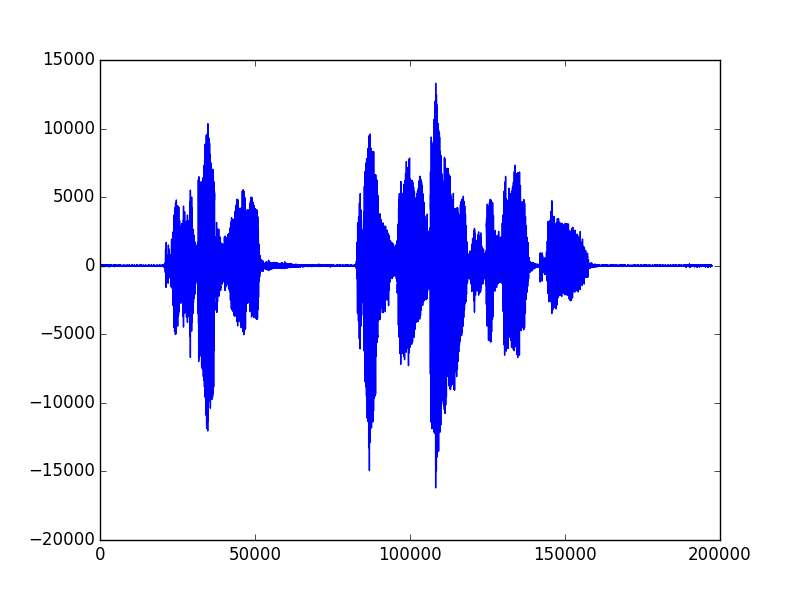
\includegraphics[width=0.5\linewidth]{images/simulation/PAR_001_original_signal}
		\caption{Original signal}
		\label{fig:PAR_001_original_signal}
	\end{figure}
	
	\begin{figure}[!th]
		\centering
		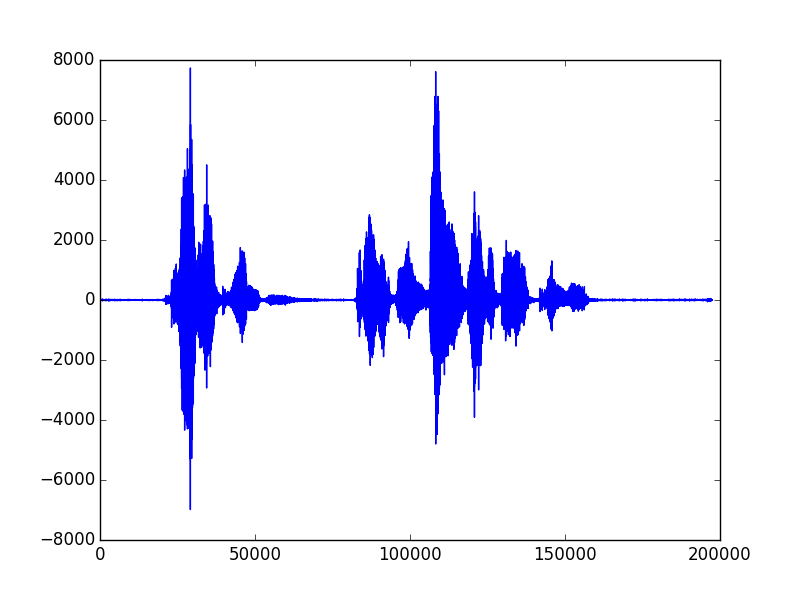
\includegraphics[width=0.5\linewidth]{images/simulation/PAR_002_preemphased_signal}
		\caption{Preemphased signal}
		\label{fig:PAR_002_preemphased_signal}
	\end{figure}

	\FloatBarrier
	\clearpage
	\subsection{Operations performed on each frame}

	\begin{figure}[!th]
		\centering
		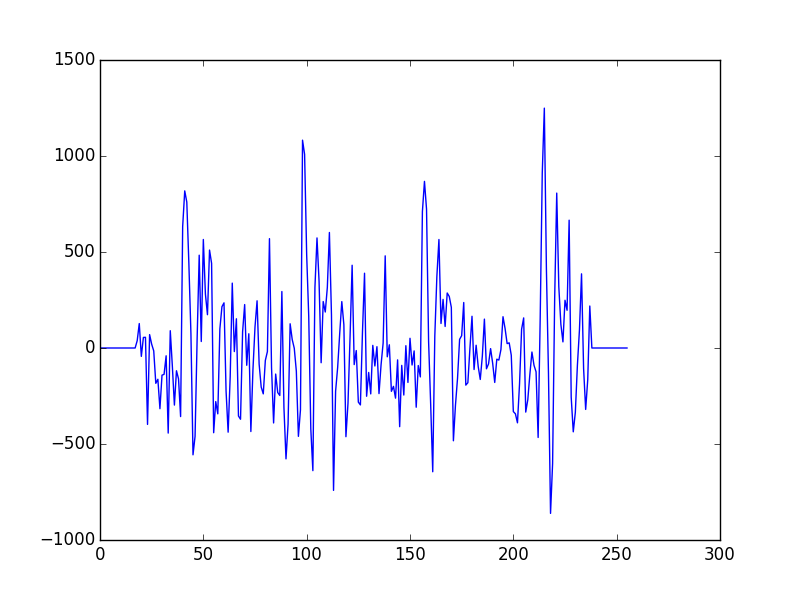
\includegraphics[width=0.5\linewidth]{images/simulation/PAR_003_padded_signal}
		\caption{Padded signal}
		\label{fig:PAR_003_padded_signal}
	\end{figure}

	\begin{figure}[!th]
		\centering
		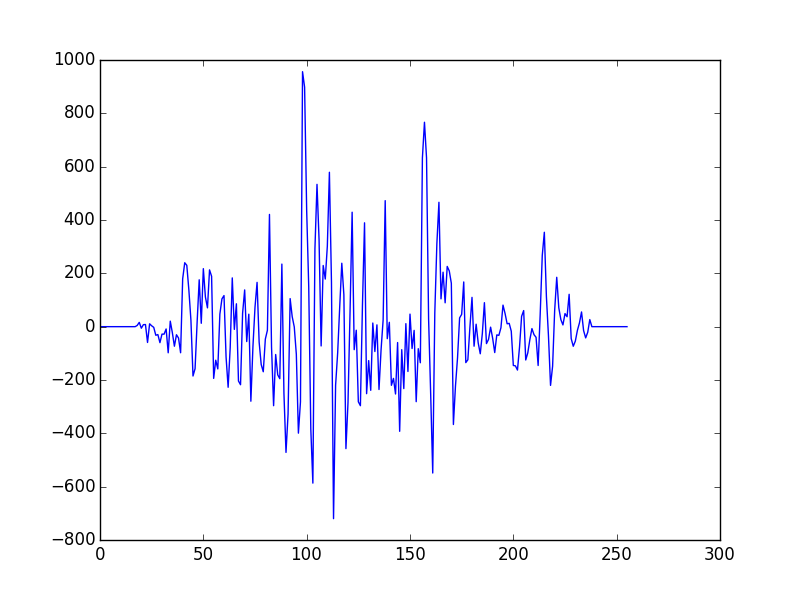
\includegraphics[width=0.5\linewidth]{images/simulation/PAR_004_windowed_signal}
		\caption{Windowed signal}
		\label{fig:PAR_004_windowed_signal}
	\end{figure}

	\begin{figure}[!th]
		\centering
		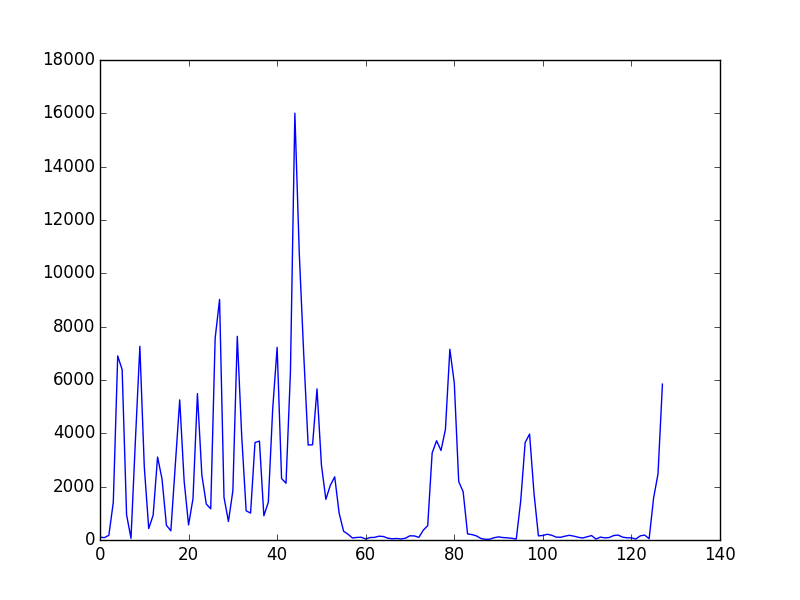
\includegraphics[width=0.5\linewidth]{images/simulation/PAR_005_after_fft_signal}
		\caption{Signal after application of \gls{FFT}}
		\label{fig:PAR_005_after_fft_signal}
	\end{figure}

	\begin{figure}[!th]
		\centering
		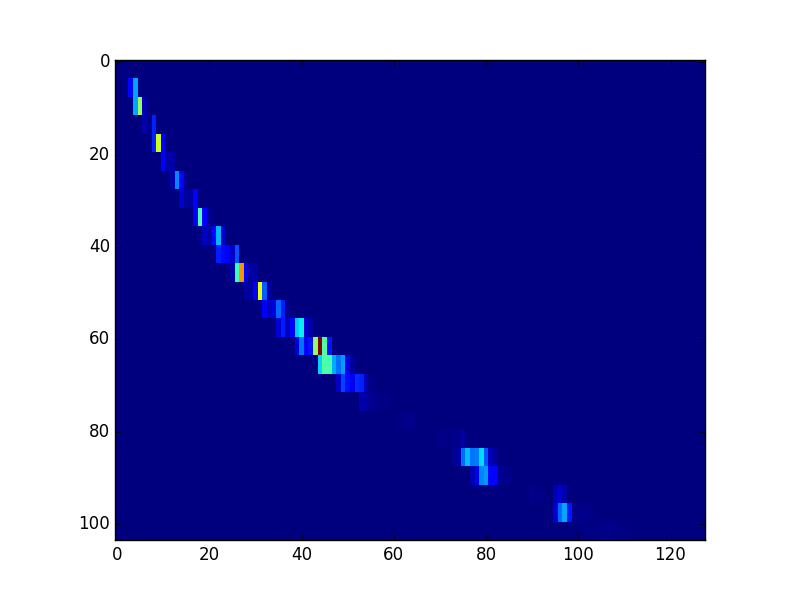
\includegraphics[width=0.5\linewidth]{images/simulation/PAR_006_mel_filtered_signal}
		\caption{Frame after mel filtering}
		\label{fig:PAR_006_mel_filtered_signal}
	\end{figure}

	\begin{figure}[!th]
		\centering
		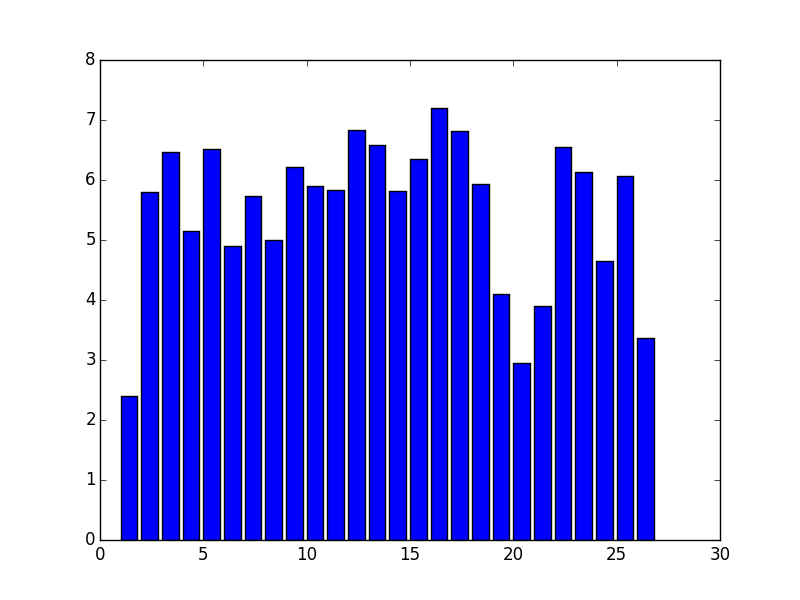
\includegraphics[width=0.5\linewidth]{images/simulation/PAR_007_mel_power_signal}
		\caption{Logarithmic power of each mel filter result}
		\label{fig:PAR_007_mel_power_signal}
	\end{figure}

	\begin{figure}[!th]
		\centering
		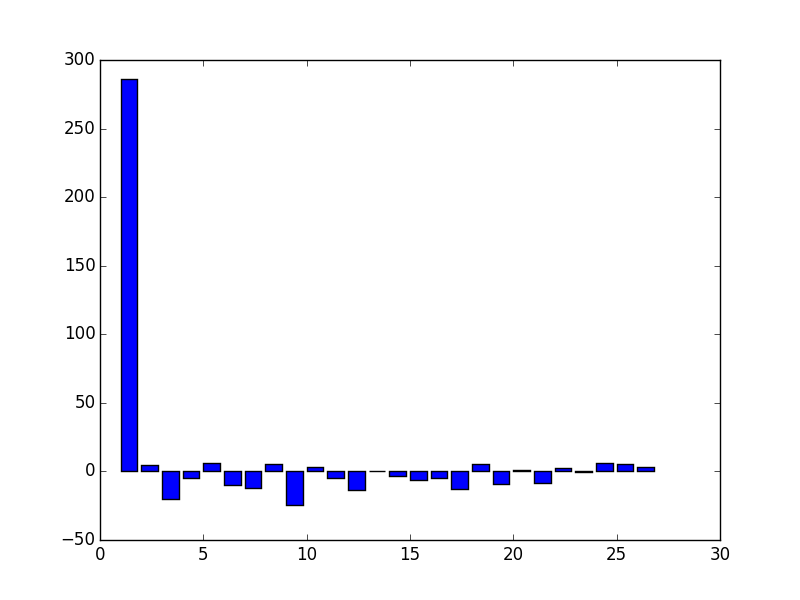
\includegraphics[width=0.5\linewidth]{images/simulation/PAR_008_cosine_transformed_signal}
		\caption{Frame after cosine transormation}
		\label{fig:PAR_008_cosine_transformed_signal}
	\end{figure}

	\FloatBarrier
	\clearpage

	\begin{figure}[th!]
		\centering
		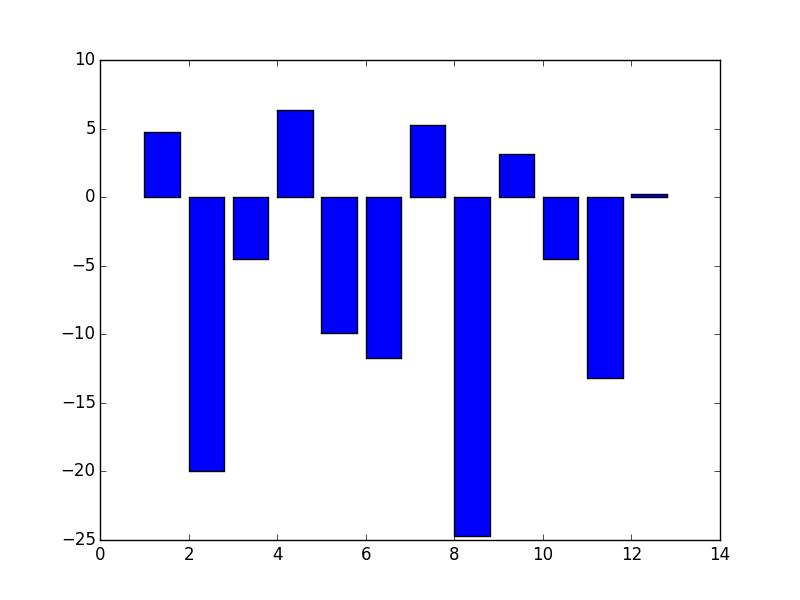
\includegraphics[width=0.5\linewidth]{images/simulation/PAR_009_liftered_signal}
		\caption{Frame after application of liftering}
		\label{fig:PAR_009_liftered_signal}
	\end{figure}

	
	\subsection{Full matrix dumps}
	\FloatBarrier
	
	\begin{figure}[th!]
		\centering
		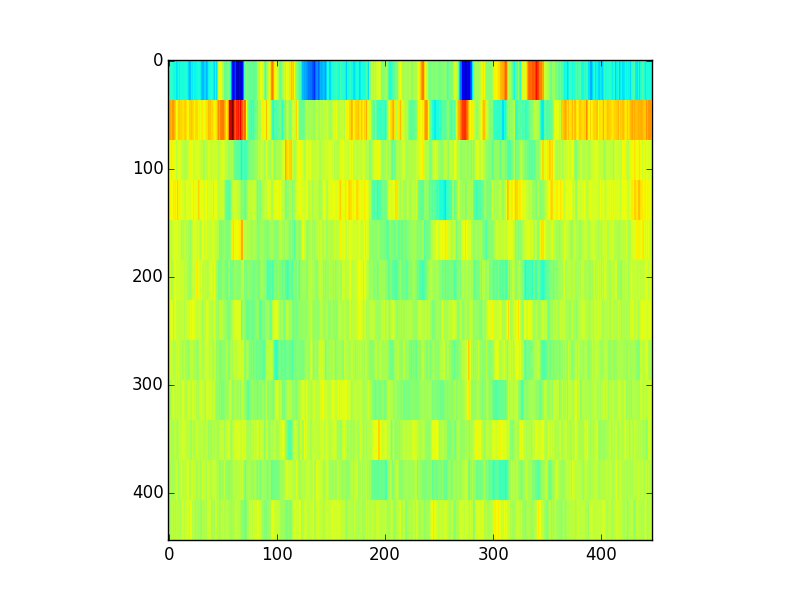
\includegraphics[width=0.5\linewidth]{images/simulation/PAR_010_parametrized_raw}
		\caption{Whole frame parametrization}
		\label{fig:PAR_010_parametrized_raw}
	\end{figure}

	\begin{figure}[th!]
		\centering
		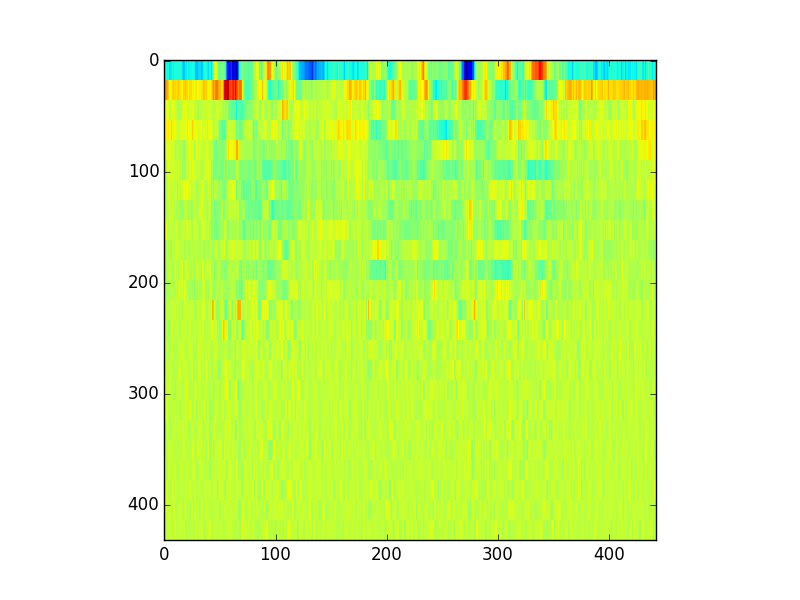
\includegraphics[width=0.5\linewidth]{images/simulation/PAR_011_parametrized_with_delta}
		\caption{Frame parametrization with deltas and deltasdeltas applied}
		\label{fig:PAR_011_parametrized_with_delta}
	\end{figure}

	\begin{figure}[th!]
		\centering
		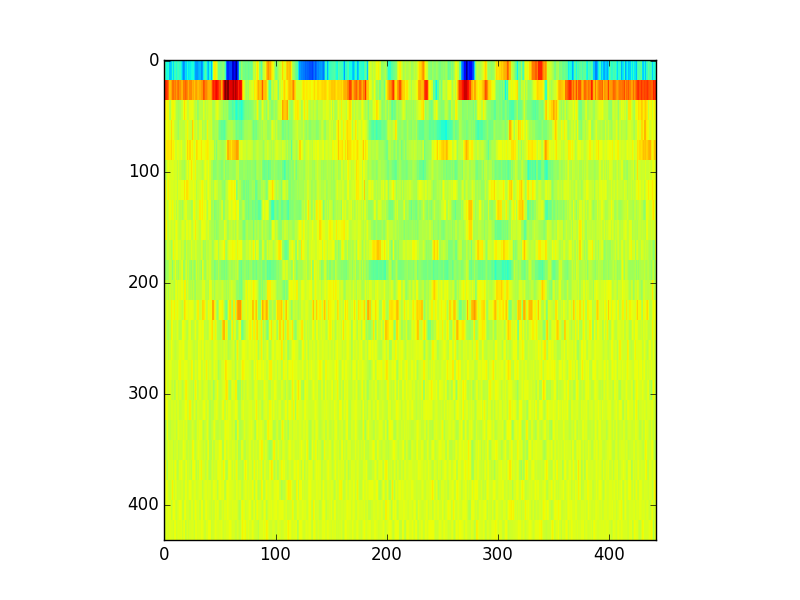
\includegraphics[width=0.5\linewidth]{images/simulation/PAR_012_feature_warped}
		\caption{Frame parametrization after feature warping}
		\label{fig:PAR_012_feature_warped}
	\end{figure}
		
	\section{Adjusting}
	
	\begin{figure}[th!]
		\centering
		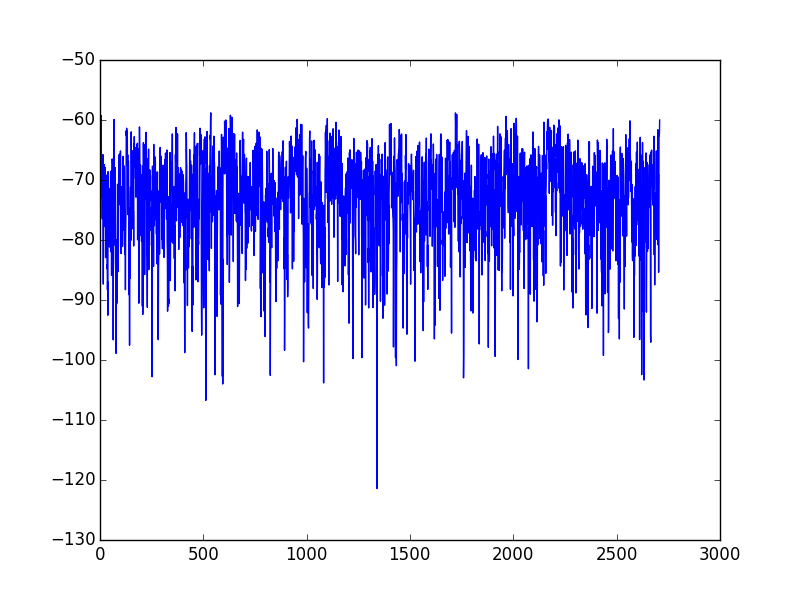
\includegraphics[width=0.5\linewidth]{images/simulation/ADJ_001_PCA_decision_output}
		\caption{Decision output of \gls{PCA} for reference data}
		\label{fig:ADJ_001_PCA_decision_output}
	\end{figure}

	\begin{figure}[th!]
		\centering
		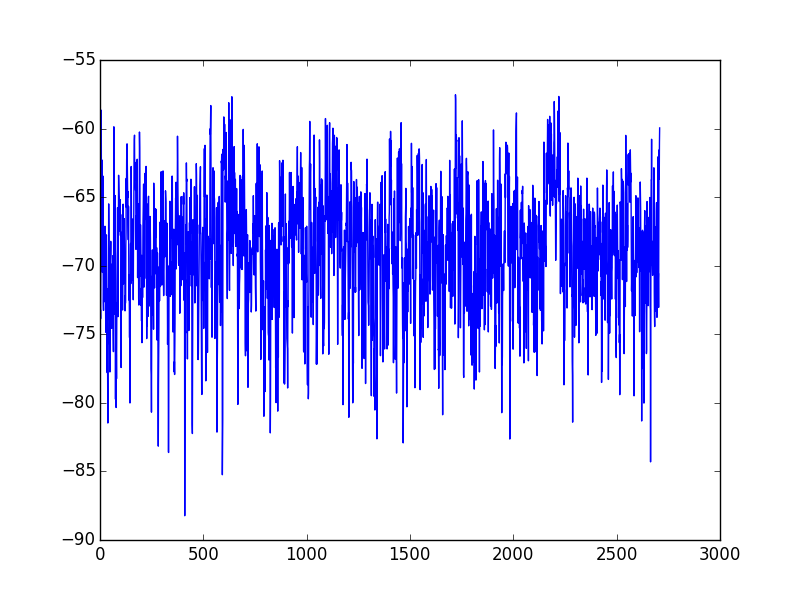
\includegraphics[width=0.5\linewidth]{images/simulation/ADJ_002_GMM_decision_output}
		\caption{Decision output of \gls{GMM} for reference data}
		\label{fig:ADJ_002_GMM_decision_output}
	\end{figure}

	
	\section{Challenging} \label{sec:challenging}
	
	\begin{figure}[th!]
		\centering
		\includegraphics[width=0.7\linewidth]{"images/simulation/CHL_001_piece_1_score of PCA"}
		\caption{Score comparison of \gls{PCA} for piece 1}
		\label{fig:CHL_001_piece_1_scoreofPCA}
	\end{figure}
	
	\begin{figure}[th!]
		\centering
		\includegraphics[width=0.7\linewidth]{"images/simulation/CHL_002_piece_1_score of GMM"}
		\caption{Score comparison of \gls{GMM} for piece 1}
		\label{fig:CHL_002_piece_1_scoreofGMM}
	\end{figure}
	
	\begin{figure}[th!]
		\centering
		\includegraphics[width=0.7\linewidth]{"images/simulation/CHL_003_piece_2_score of PCA"}
		\caption{Score comparison of \gls{PCA} for piece 2}
		\label{fig:CHL_001_piece_2_scoreofPCA}
	\end{figure}
	
	\begin{figure}[th!]
		\centering
		\includegraphics[width=0.7\linewidth]{"images/simulation/CHL_004_piece_2_score of GMM"}
		\caption{Score comparison of \gls{GMM} for piece 2}
		\label{fig:CHL_002_piece_2_scoreofGMM}
	\end{figure}

	\FloatBarrier

	In figures \ref{fig:CHL_001_piece_1_scoreofPCA}-\ref{fig:CHL_002_piece_2_scoreofGMM} it can be easily seen that speaker 1 reaches always the highest score. Moreover speaker 3 gets higher score then speaker 2 since 1 and 3 are both male. These relations can be also seen in console output, where average score for each case is given:\\
	
	\inputminted{bash}{images/simulation/AAA_console_out}
	
	\chapter{Conclusion}

	As it was shown section \ref{sec:challenging} the presented method gives satisfying results. However much more tests should be executed in order to assure proper reliability of system constructed on this library.\\
	
	It is also worth mentioning that all of applied classification methods in this thesis where basing on only one class of input samples. Methods like \gls{SVM} or artificial neural networks require samples that belong and \underline{not} belong to desired set. It basically means that collecting large database of audio samples lets to improve accuracy of these detections. Therefore the mostly guarded part of commercial systems used for speaker recognition are not just algorithms, but huge database collected over years of building such system.\\
	
	Another step of developing this library could be collecting large test data set and try to adjust all of the parameters in order to provide optimal results. It could be also worth considering to add some new classification algorithms and invent some probabilities combining function. After having this library tested and considered as reliable one could try to implement all of these algorithms on real digital signal processor or microcontroller in order to construct some commercial device used for voice authorization. One could simply rewrite this library to some low level programming language that would compute all of these operations much faster, then this theoretical model.

	\appendixpage	
	\appendix
	
	\chapter{Source code of SignalParametrizer class} \label{ch:impl_signal_param}

	\inputminted[linenos=true]{python}{../automatic_speaker_recognition/src/processing/signalparametrizer.py}
	
	\chapter{Source code of Classifier class} \label{ch:impl_classifier}
	
	\inputminted[linenos=true]{python}{../automatic_speaker_recognition/src/processing/classifier.py}
	
	\nocite{*}
	\bibliographystyle{dyplom}
	\bibliography{bibliography}

\end{document}
